\documentclass{article}
\usepackage{graphicx}
\graphicspath{ {./gambar/} }

\title{Laporan Python}
\author{Naomi C.H Tampubolon }
\date{October 2019}

\begin{document}

\maketitle

\section{Python}
Sebelum kita  membahas sejarah Python, kita membahas apa itu Python? Python adalah bahasa pemrograman interpretatif multiguna dengan filosofi perancangan yang berfokus pada tingkat keterbacaan kode. Sebagai bahasa pemrograman Python dikatakan dapat menggabungkan kapabilitas, kemampuan, dengan sintaksis kode yang sangat jelas, serta dilengkapi dengan fungsionalitas pustaka standar yang besar serta komiprehensif. Python juga didukung oleh komunitas yang besar.
Dalam sejarahnya, Python pertama kali diciptakan oleh Guido van Rossum di Centrum Wiskunde & Informatika (CWI) di Belanda pada awal tahun 1990-an.  Bahasa ini terinspirasi dari bahasa pemrograman ABC. Di tahun 1995, Guido merilis beberapa versi dari Python. Versi python yang dirilis bersifat open source dan hampir semua menggunakan lisensi GFL-compatible. Nama Python ini sendiri berasal dari nama grup komedi terkenal di Inggris bernama Monty Python, lalu kemudian ia memberi nama bahasa ciptaannya dengan nama Python.

Berikut adalah versi mayor dan minor python:
\begin{itemize}
\item Python 1.0 - Januari  1994\\
Python 1.2 - 10 April 1995\\
Python 1.3 - 12 Oktober 1995\\
Python 1.4 - 25 Oktober 1996\\
Python 1.5 - 31 Desember 1997\\
Python 1.6 - 5 September 2000
\item Python 2.0 - 16 Oktober 2000\\
Python 2.1 – 17 April 2001\\
Python 2.2 – 21 Desember 2001\\
Python 2.3 – 29 Juli 2003\\
Python 2.4 – 30 Nopember 2004\\
Python 2.5 – 19 September 2006\\
Python 2.6 – 1 Oktober 2008\\
Python 2.7 – 3 Juli 2010
\item Python 3.0 – 3 Desember 2008\\
Python 3.1 – 27 Juni 2009\\
Python 3.2 – 20 Februari 2011\\
Python 3.3 – 29 September 2012\\
Python 3.4 – 16 Maret 2014\\
Python 3.5 – 13 September 2015\\
Python 3.6 – 23 Desember 2016\\
Python 3.7 – 27 Juni 2018
\end{itemize}
Python versi 2 dan python versi 3, kedua versi python ini memiliki beberapa perbedaan dalam penulisan skripnya. Berikut adalah perbedaan Python 2 dan Python 3 yang mendasar:

\begin{enumerate}
\item \textbf{Print}.
\begin{itemize}
\item Pada python2, print diperlakukan seperti statemen daripada sebuah function.\\ 
1. print "Aku anak Indonesia"
\item Pada python 3, print diperlakukan sebagai function.\\
1. print("Aku anak Indonesia")
\end{itemize}
Perubahan ini membuat sintaksis python lebih konsisten. Python 2.7 juga kompatibel dengan penggunaan print().
\item \textbf{Pembagian pada Integer}
\begin{itemize}
\item Pada python 2, tipe data angka yang tidak mengandung atau bukan desimal akan diperlakukan sebagai integer. Ketika membagi kedua integer akan didapatkan tipe data float. Python 2 menggunakan floor division atau akan dibulatkan ke nilai paling rendah, misalnya 1,5 menjadi 1. Pada python 2.7 akan menjadi seperti ini:\\
x = 3 / 2\\
print x\\
Output\\
1\\
Untuk desimal maka tambahkan, seperti ini 3,0 / 2,0 untuk mendapatkan hasil 1,5
\item Pada python 3, pembagian pada bilangan integer intuitif, kita juga dapat melakukan 3,0 / 2,0 untuk hasil 1,5 tapi untuk mendapatkan nilai floor division maka pada python 3 gunakan "//":\\
b = 3 // 2\\
print(b)\\
Output\\
1
\end{itemize}
\item \textbf{Dukungan Unicode}
\begin{itemize}
\item Python 2 menggunakan alfabet ASCII secara default, sehingga ketika kita mengetik “Halo!”  maka Python 2 menangani string sebagai ASCII. Terbatas pada beberapa ratus karakter, ASCII mungkin bukan pilihan yang fleksibel untuk menangani proses encoding terutama yang non English. Untuk menggunakan unicode yang lebih luwes, mendukung lebih dari 128,000 karakter maka kita harus mengetik u”Halo!” , dengan tambahan u  di depannya yang mana berarti Unicode.
\item Python 3 menggunakan Unicode secara default, yang mana menyelamatkan programmer dari tambahan kode lagi, lebih hemat waktu dan mudah untuk diisikan dan ditampilkan. Karena Unicode mendukung berbagai karakter linguistik yang beragam termasuk menampilkan emoji, penggunaan karakter secara default dengan encoding memastikan perangkat mobile didukung oleh program yang kita buat.
\end{itemize}
\end{enumerate}

\section{Python dalam Dunia Pekerjaan}
Spotify adalah sebuah flatform yang telah memanfaatkan python dalam analisis data. Pemanfaatan ini terlihat jelas pada bagaimana Spotify merekomendasikan lagu kepada pelanggannya. Berikut beberapa poin-poin tentang penggunaan python dalam analisis data Spotify:
\begin{enumerate}
\item Tim Spotify memanfaatkan analitis. Mereka memanfaatkan Luigi, modul dari Python, yang disinkronisasi dengan Hadoop, sebuah framework berbasis Java yang memungkinkan pemrosesan data dengan ukuran sangat besar.
\item Luigi memungkinkan kamu untuk membangun pipeline yang kompleks dengan cepat. Ini menangani bundling library yang dibutuhkan, serta mengembalikan error log ke komputer lokalmu.
\item Spotify juga mengaplikasikan Luigi bersama dengan berbagai algoritme machine learning untuk menghidupkan fitur Radio dan Discover, serta rekomendasi untuk orang yang mungkin ingin kamu ikuti.
\item Di laman Spotify Labs, Spotify menyatakan bahwa mereka menggunakan bahasa pemrograman Python dalam sembilan puluh persen urusan MapReduce mereka. Data Science Graduate Program mengibaratkan Hadoop sebagai sumber hidup big data, sementara MapReduce berperan sebagai detak jantungnya.	
\end{enumerate}

\section{Instalisasi Python}
Instalasi python di windows sangat mudah, tapi ada konfigurasi yang harus dipilih ditengah-tengah proses instalasi, agar perintha python dapat dikenali di CMD. Python yang akan di install kali ini adalah python versi 3.7.4.

\begin{itemize}
\item Pertama download python di situs resmi python. (https://www.python.org/downloads/windows/).\ref{web.png}
\begin{figure}[!htbp]
	\centering
	\includegraphips[width=10cm]{figures/web.png}
	\caption{Situs Resmi Python}
\end{figure}
\item Buka file python yang telah di download tadi. Klik kanan lalu Run as Administrator.\ref{open.png}
\begin{figure}[!htbp]
	\centering
	\includegraphips[width=10cm]{figures/open.png}
	\caption{Install Python}
\end{figure}
\item Pilih "Install Now", jangan lupa centang "Install launcher for all users" agar dapat dipakai untuk semua pengguna di komputer anda. Centang juga "Add python 3.7 to path" agar perintah python dapat dikenali pada Command Prompt.\ref{cust.png}
\begin{figure}[!htbp]
	\centering
	\includegraphips[width=10cm]{figures/cust.png}
	\caption{Kostumisasi python}
\end{figure}
\item Tunggu proses sampai selesai.\ref{proses.png}
\begin{figure}[!htbp]
	\centering
	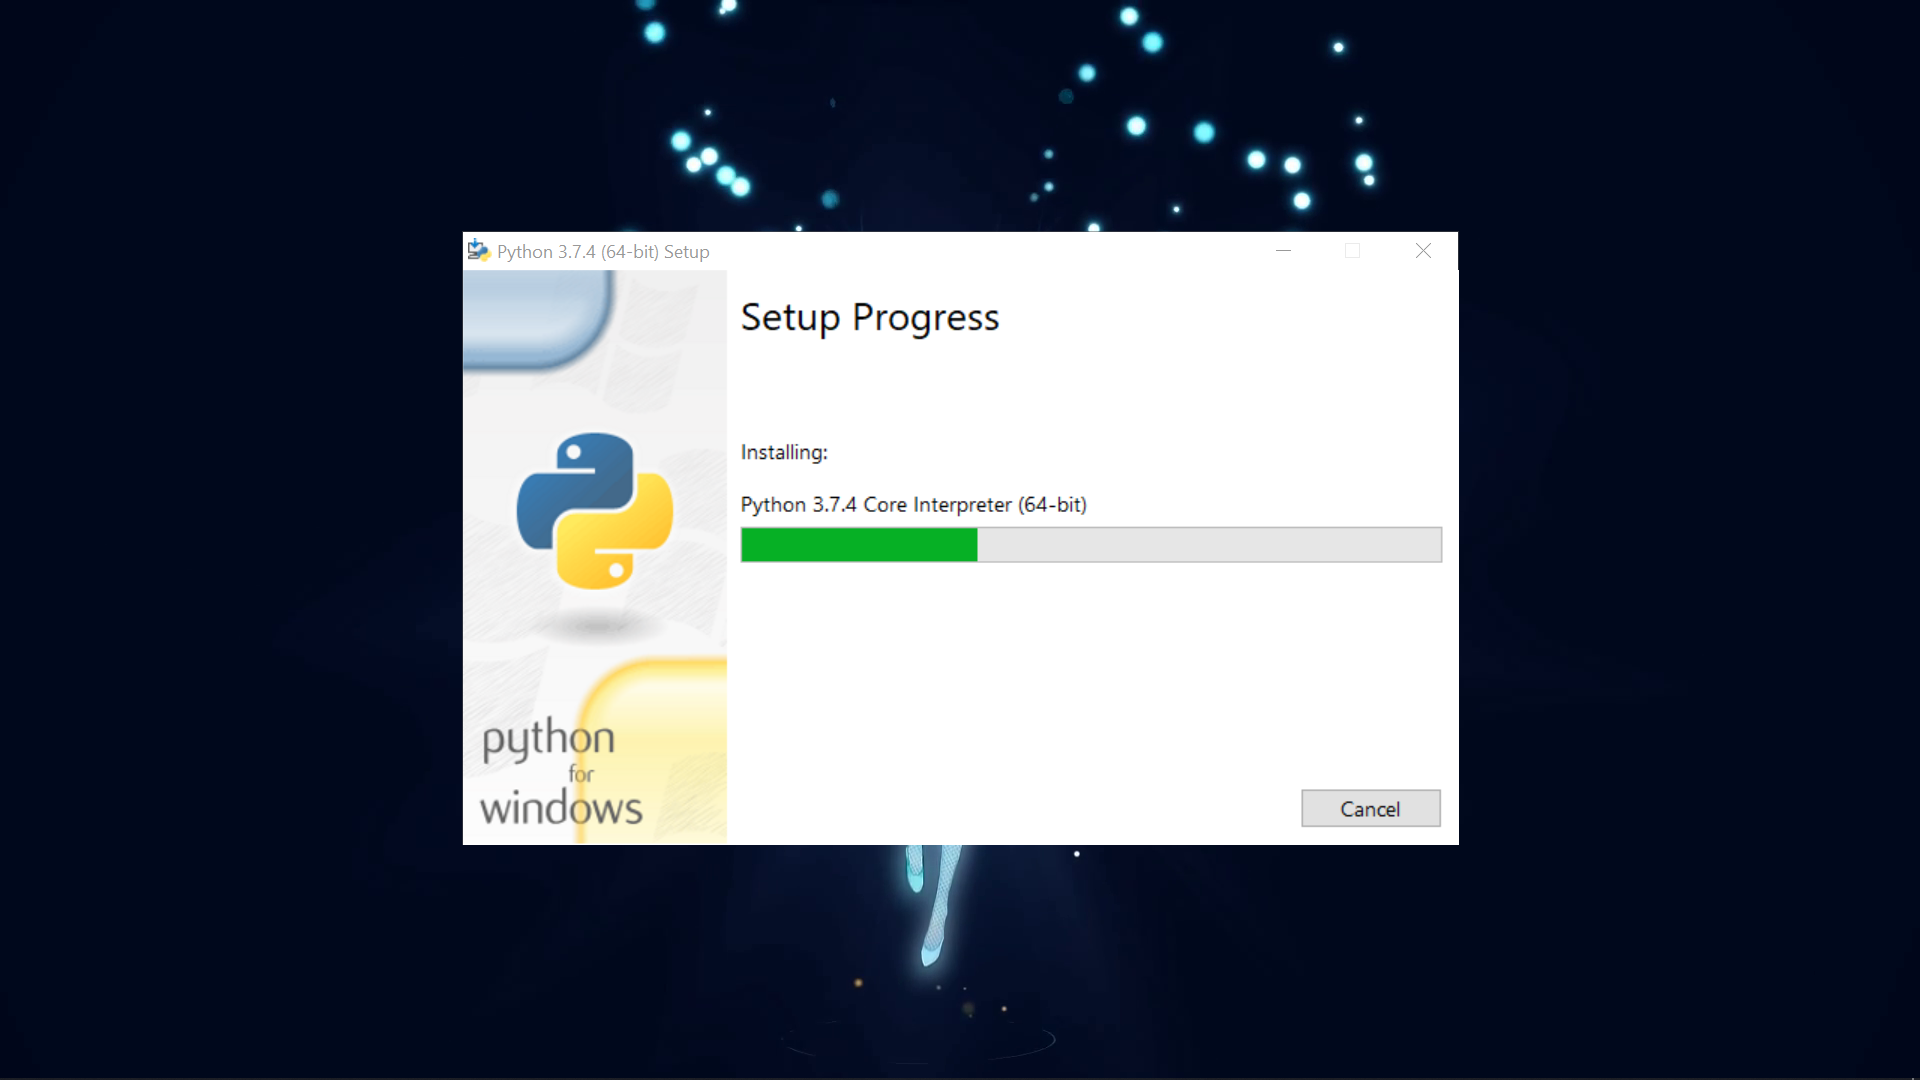
\includegraphics[width=10cm]{figures/pro.png}
	\caption{Proses Instalasi}
\end{figure}
\item Jika sudah selesai klik "Close" saja.\ref{finish.png}
\begin{figure}[!htbp]
	\centering
	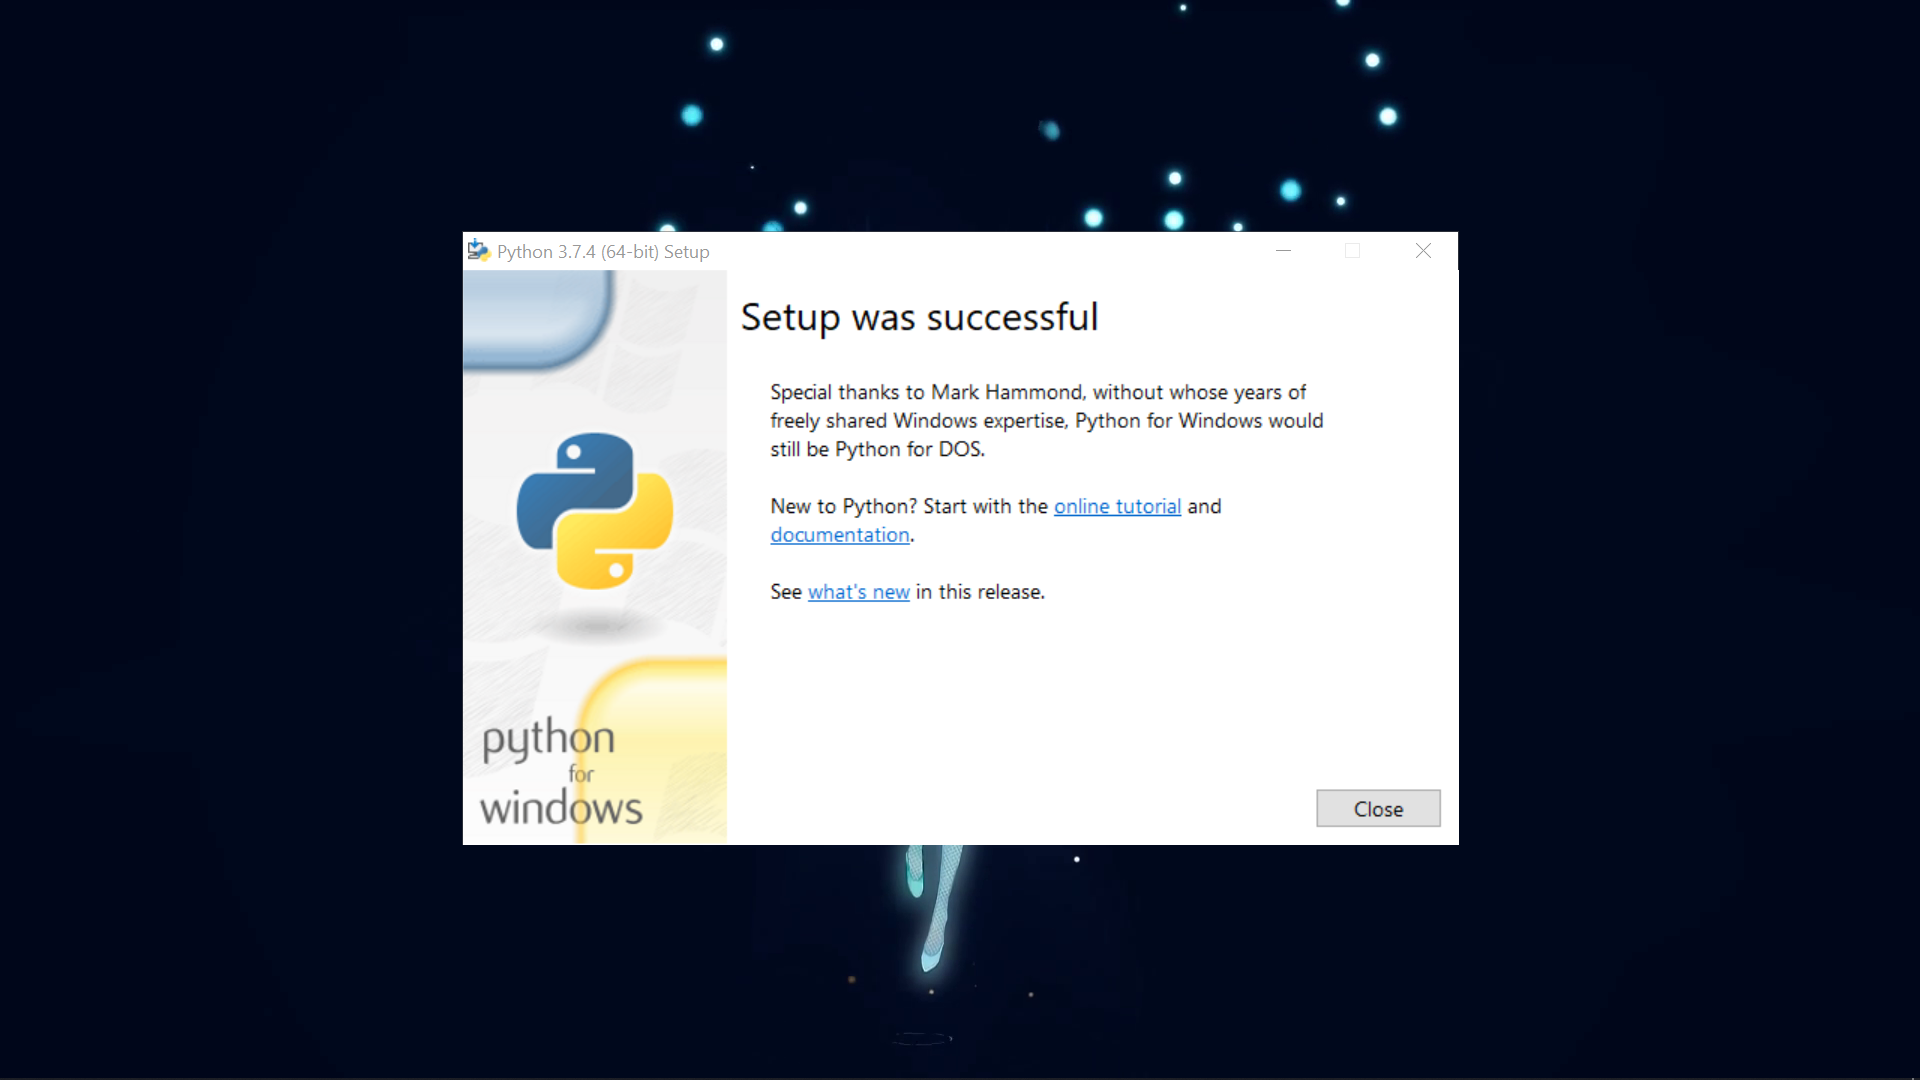
\includegraphics[width=10cm]{figures/finish.png}
	\caption{Proses Instalasi Selesai}
\end{figure}
\end{itemize}

\Section{Install pip}
Secara default pip akan terinstall pada python versi 2.7.9 keatas dan python versi 3.4 keatas, namun jika di device anda terinstall versi terbaru maka anda harus menginstall secara manual. Karena disini kita menggunakan python versi 3.7.4, jadi pip telah terinstall di dalam windows kita, tapi jika menggunakan python versi 2.7.9 dan python versi 3.4 kebawah anda harus menginstall pip secara manual. Berikut cara menginstall pip secara manual.

\begin{itemize}
\item Download pip di website resminya, anda akan mendownload file setup yakni get-pip.py dengan cara klik kanan pada linknya dan pilih "Save Link as..", nah file ini yang menjadi master instalasi pip2.
\begin{figure}[!htbp]
	\centering
	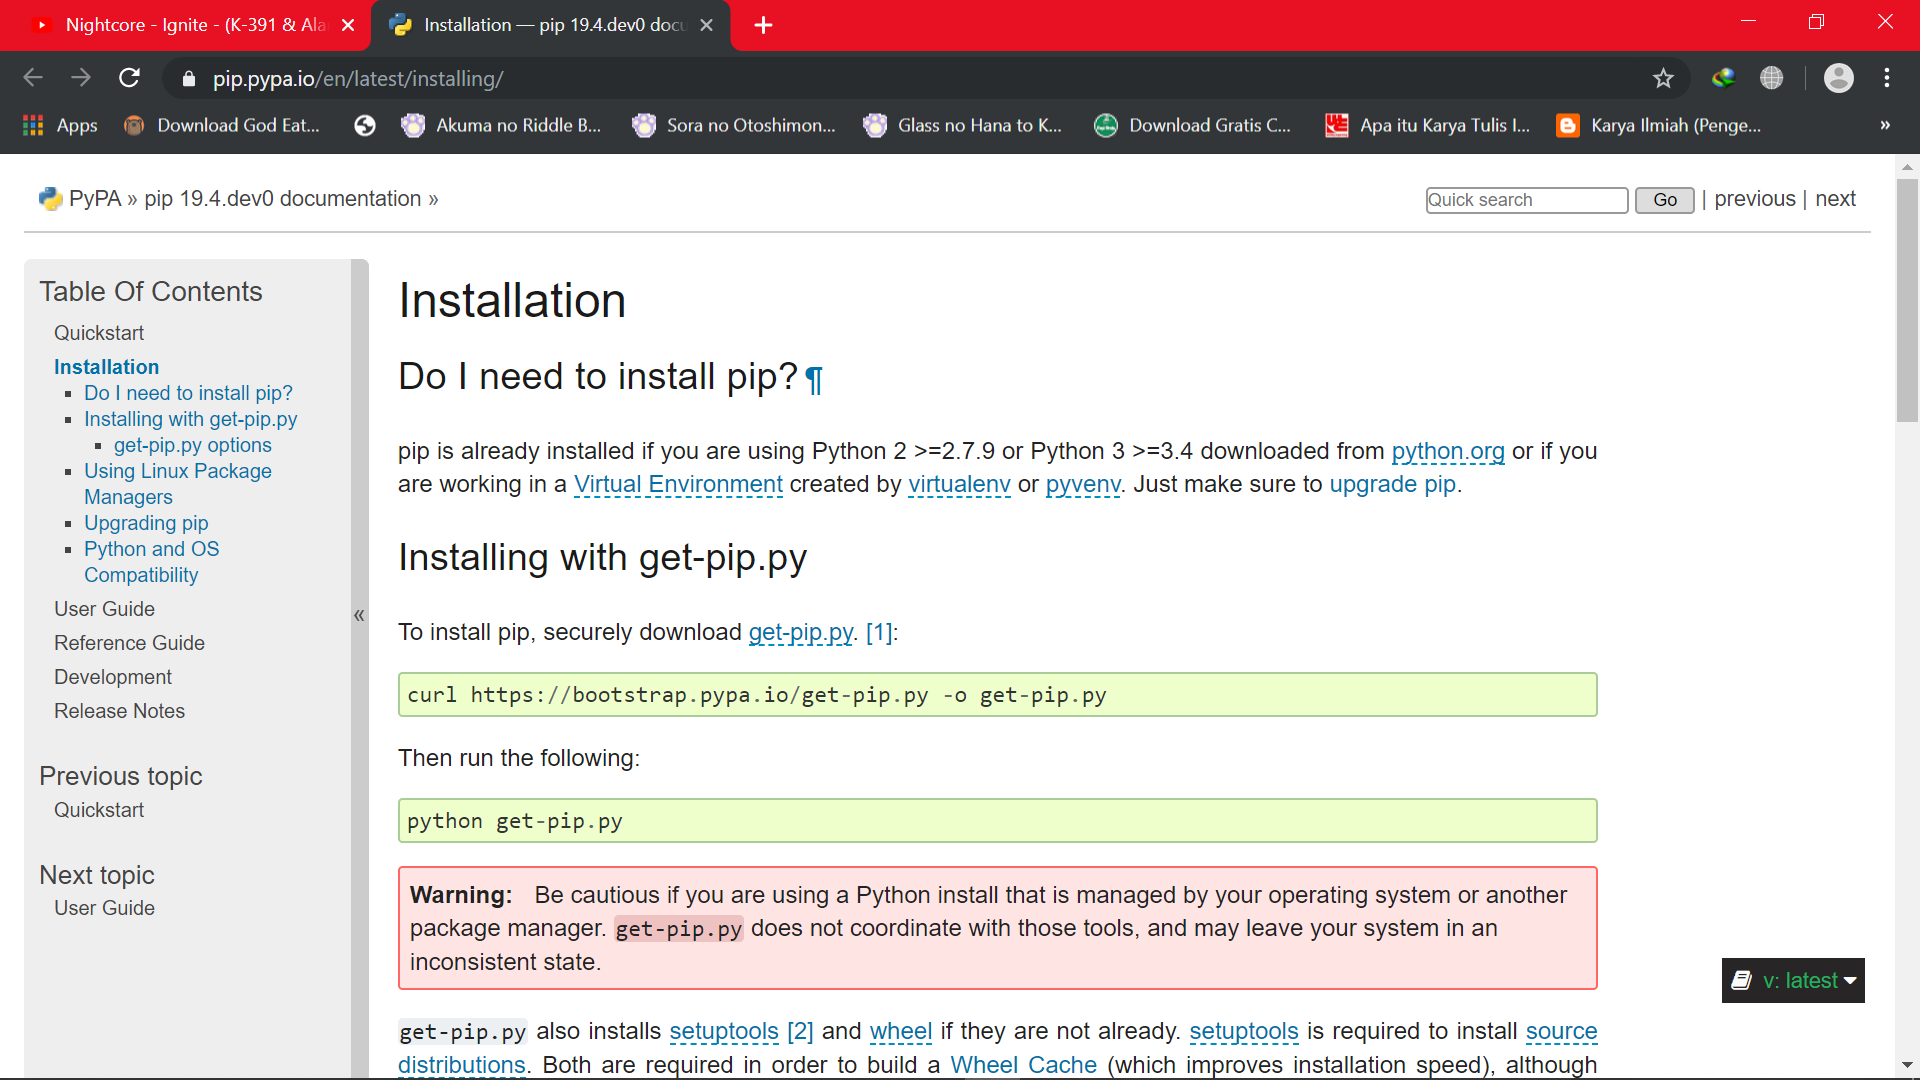
\includegraphics[width=10cm]{figures/getpip.png}
	\caption{Mendapatkan Pip}
	\label{getpip.png}
\end{figure}
\item Pindahkan file get-pip.py ke direktori yang mudah terjangkau. Lalu klik dua kali pada file get-pip.py dan pip akan terinstall dengan sendirinya.\ref{inspip.png}
\begin{figure}[!htbp]
	\centering
	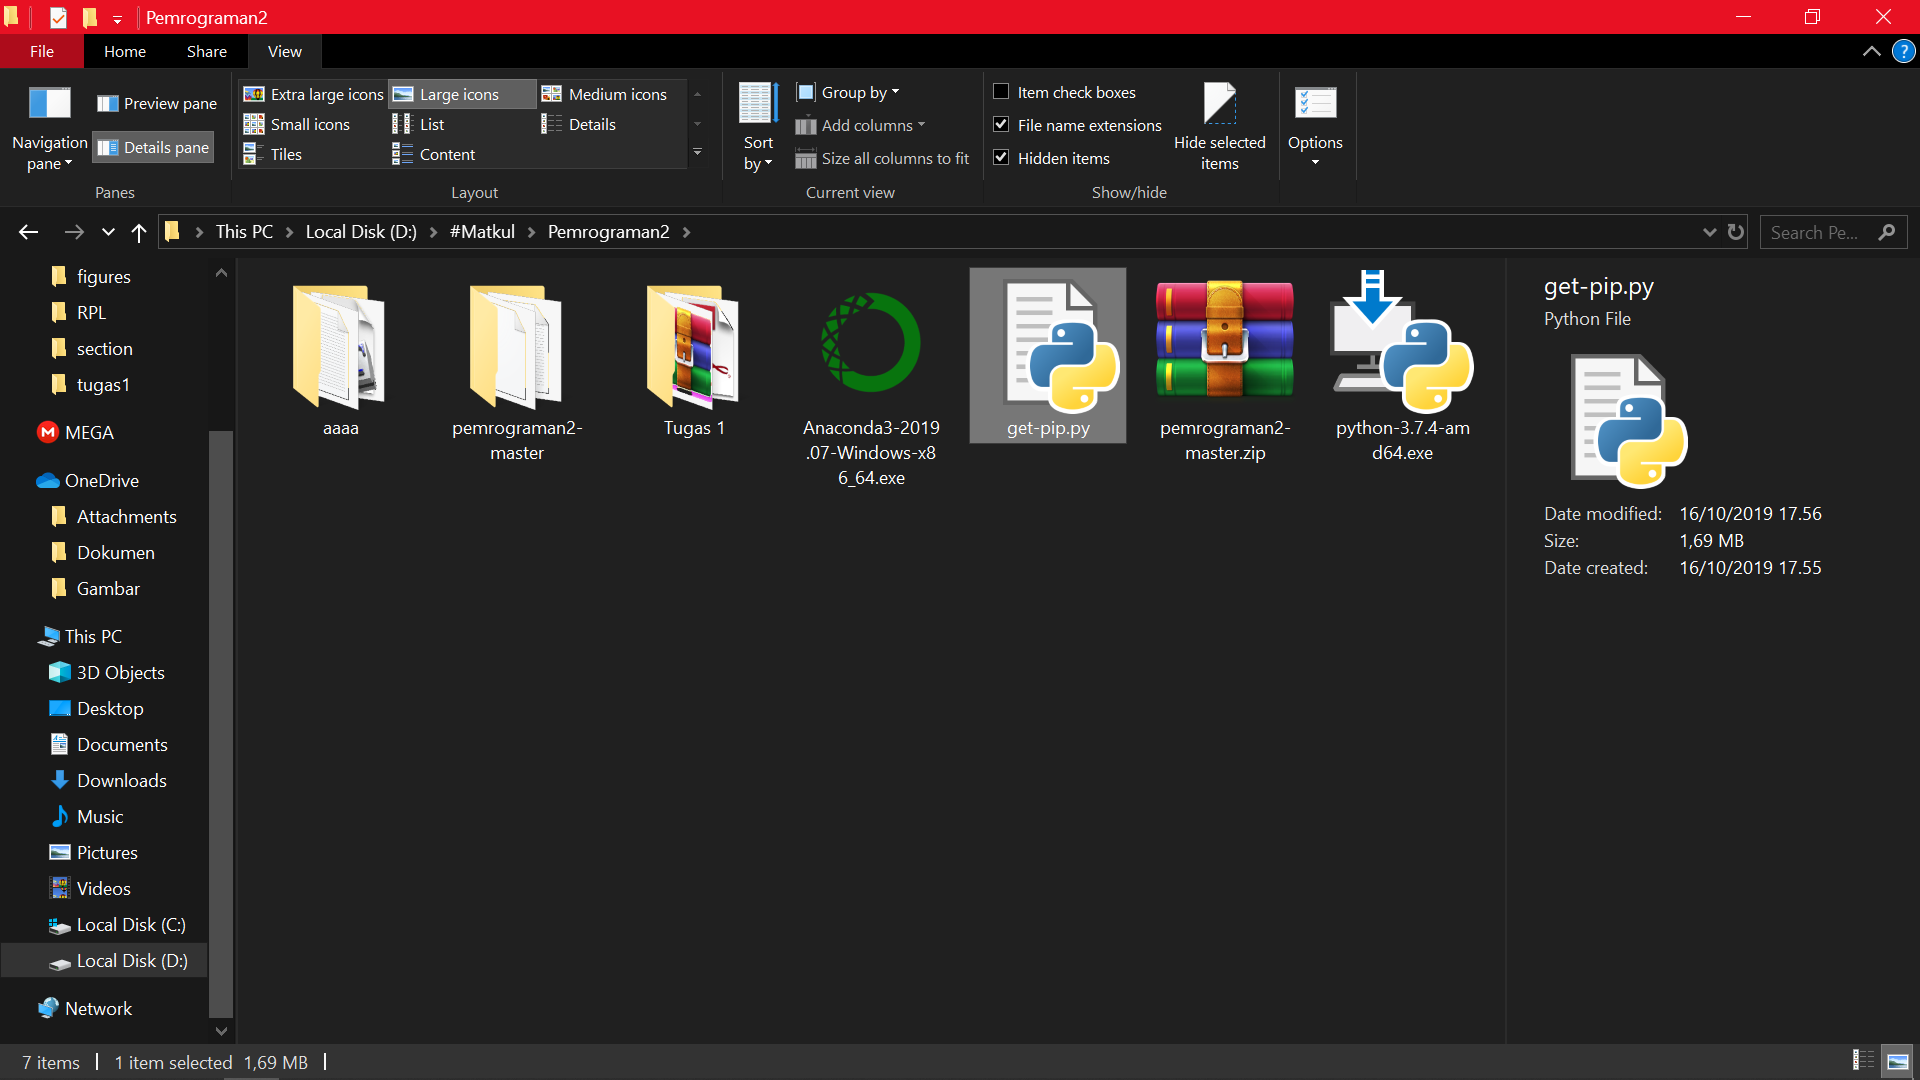
\includegraphics[width=10cm]{figures/inspip.png}
	\caption{Install PIP}
	\label{inspip.png}
\end{figure}
\end{itemize}

\section{Setting Environment}
Setting environment ini berguna agar python dapat diakses lewat CMD (Command Prompt). Berikut adalah cara mengatur environment di windows:

\begin{itemize}
\item Pertama masuk ke Control Panel -> System And Security -> System -> Advanced System Settings. Klik Advanced System Settings.
\begin{figure}[!htbp]
	\centering
	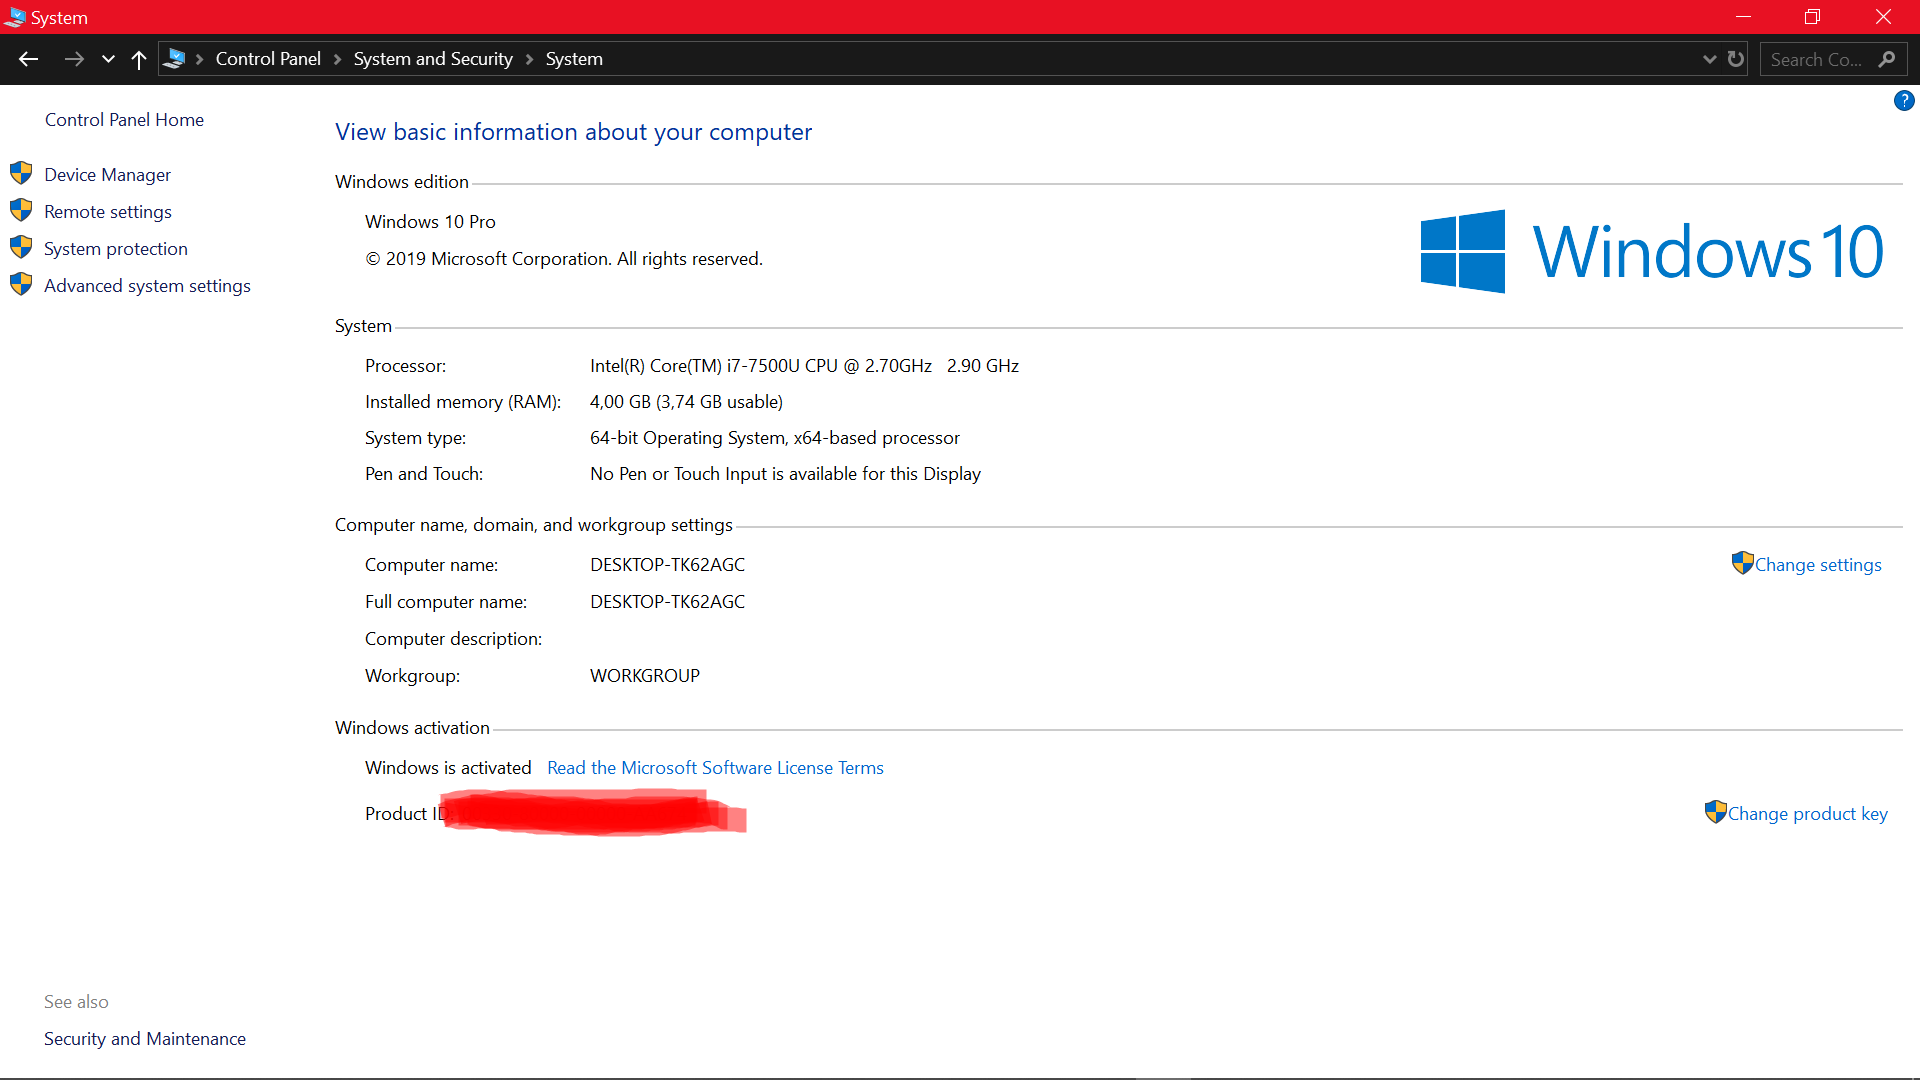
\includegraphics[scale=0.5]{figures/envi1.png}
	\caption{Computer Properties}
\end{figure}
\item Akan muncul windows baru, klik Environment variables.
\begin{figure}[!htbp]
	\centering
	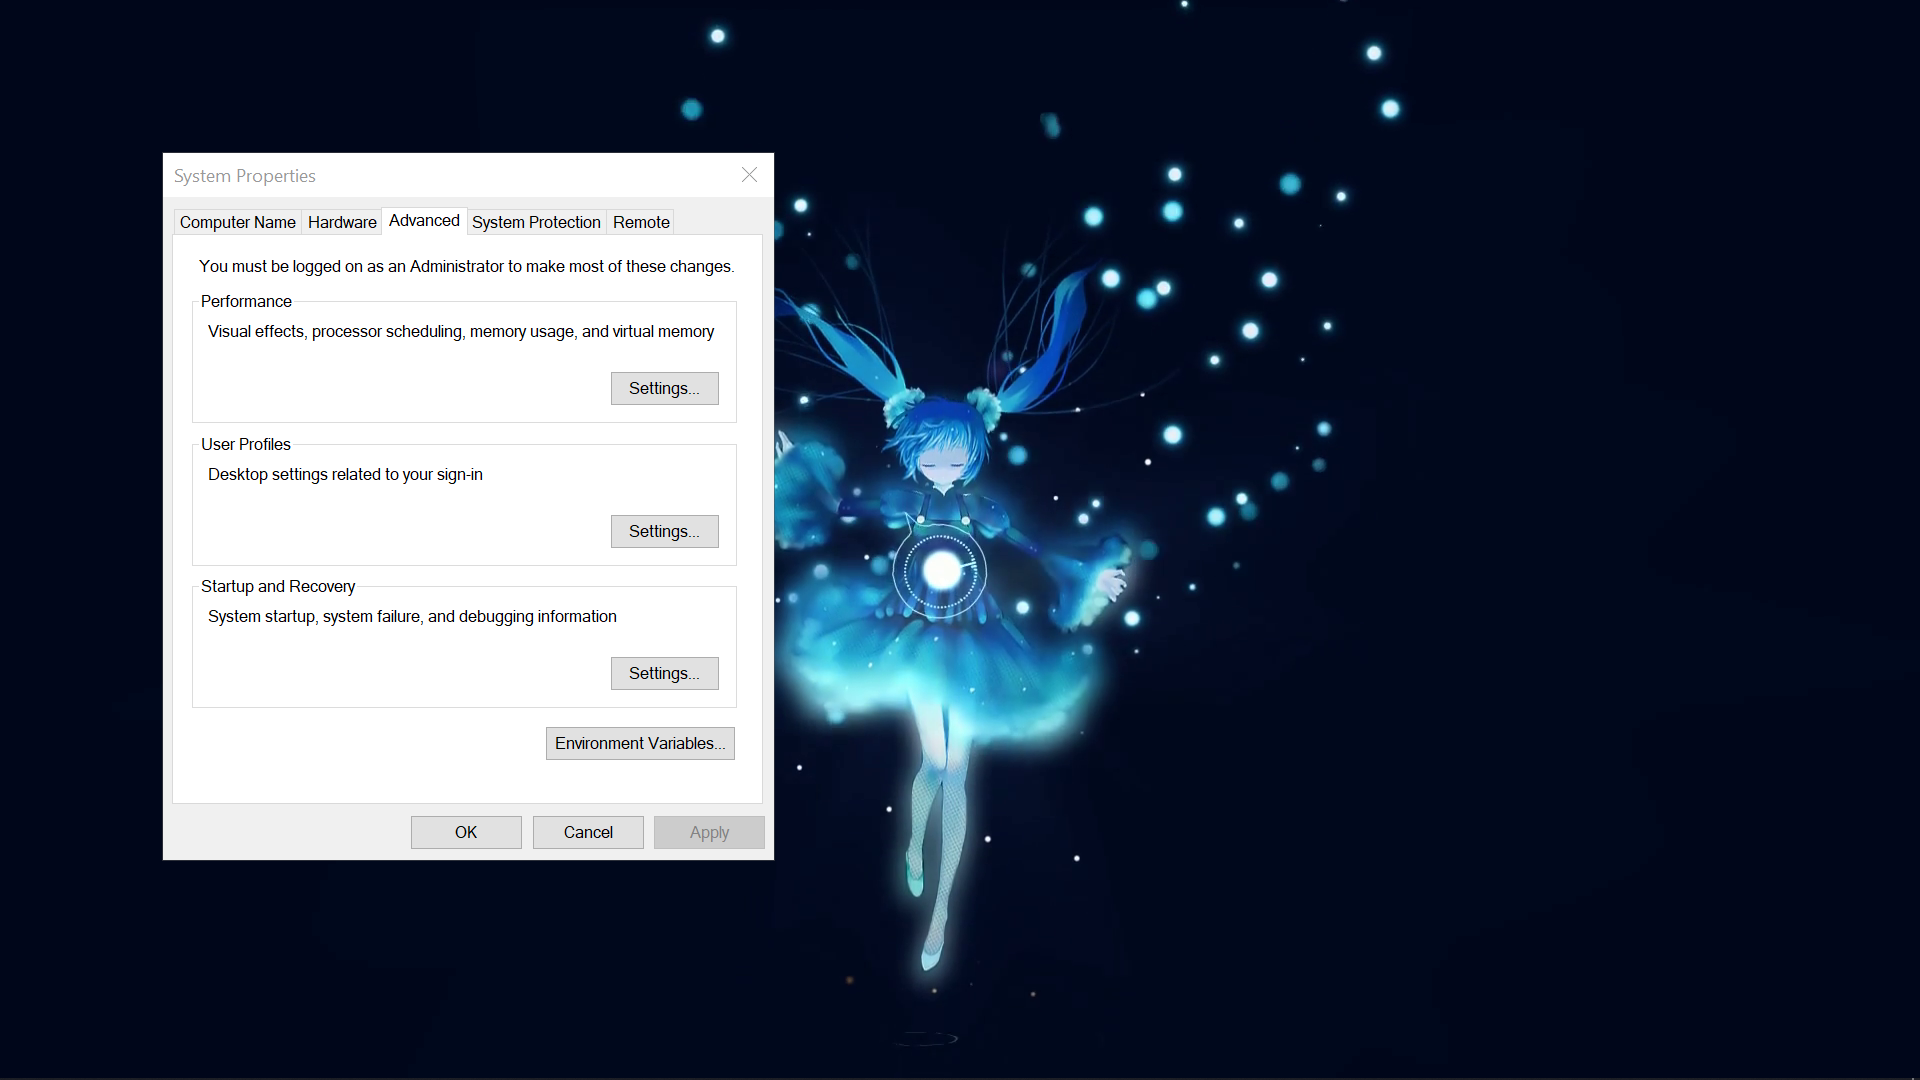
\includegraphics[scale=0.5]{figures/envi2.png}
	\caption{System Properties}
\end{figure}
\item Akan muncul windows baru, pada System Variables pilih path lalu edit.
\begin{figure}[!htbp]
	\centering
	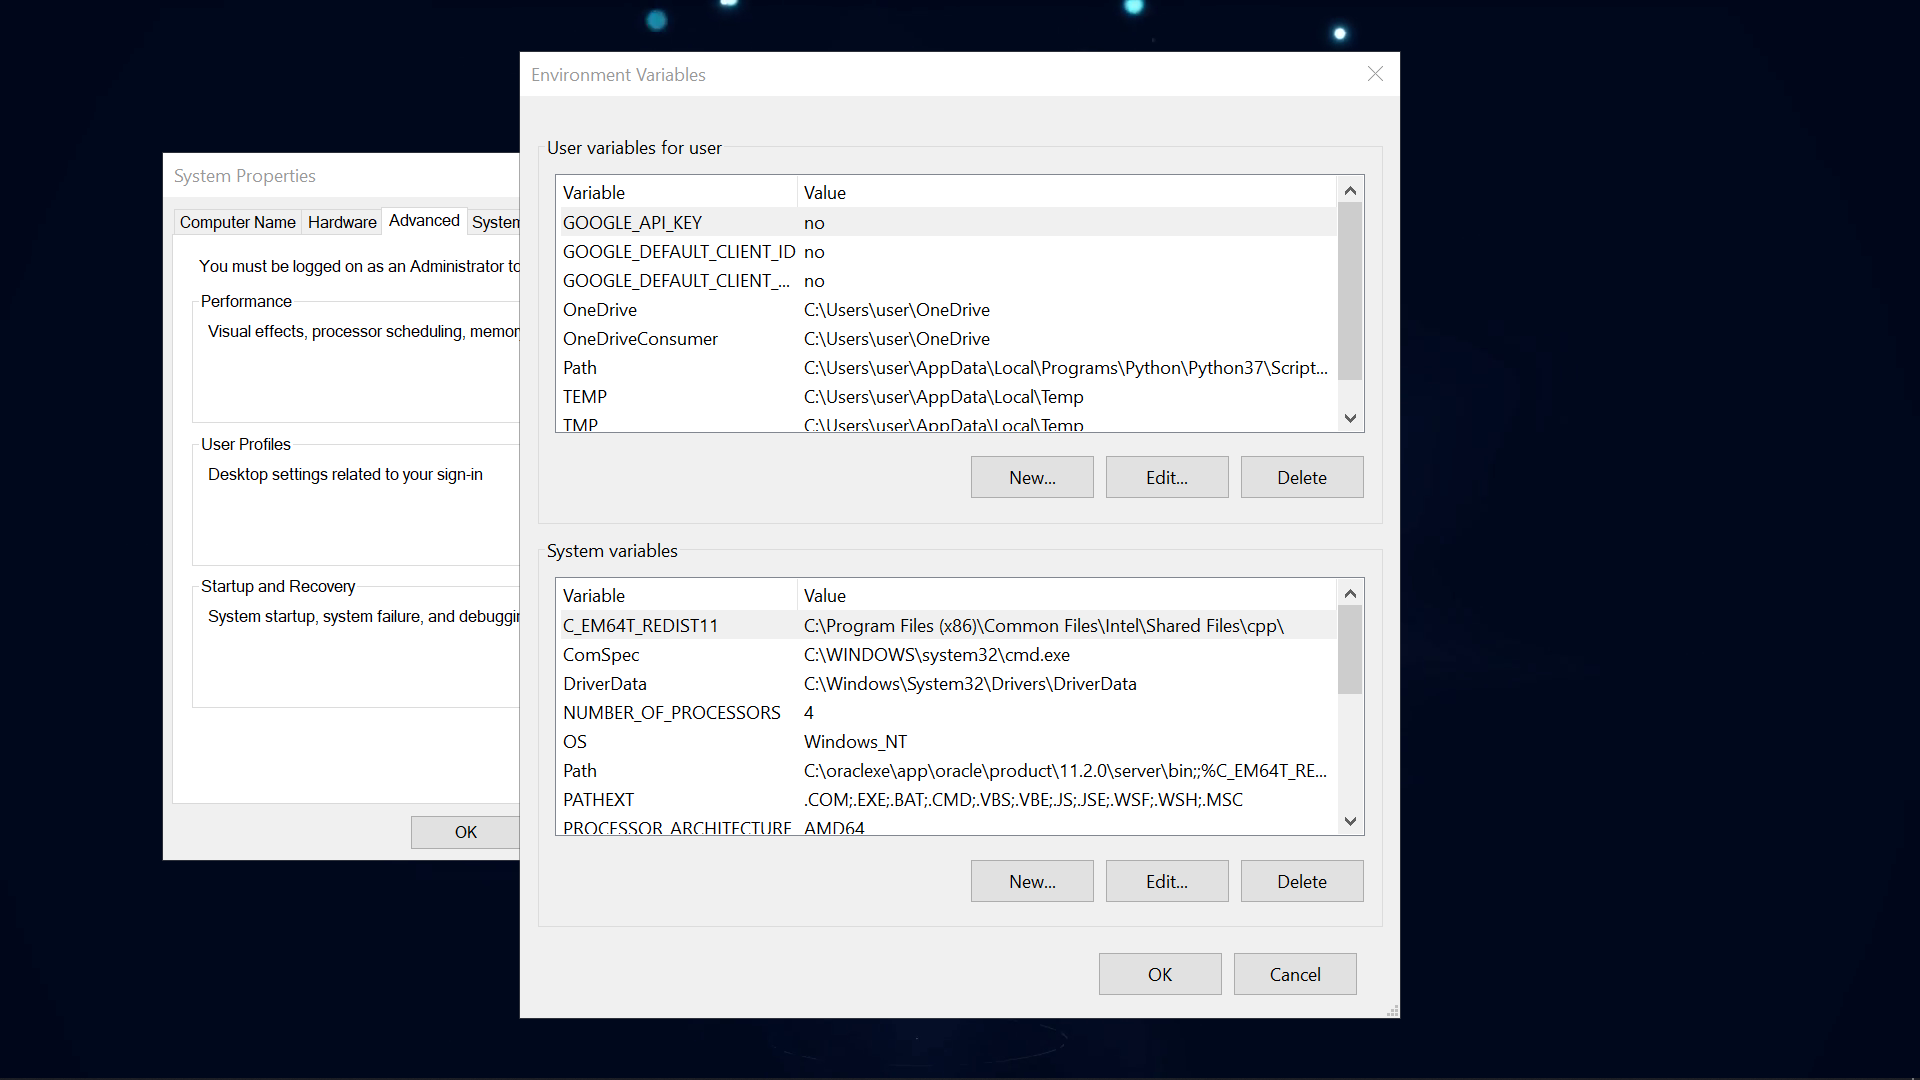
\includegraphics[width=10cm]{figures/envi3.png}
	\caption{System Variabels}
\end{figure}
\item Akan muncul windows baru, klik new lalu tambahkan Python37/scripts. Sesuaikan dengan direktori installasi python. Dalam kasus saya, saya menyimpannya sesuai dengan yang tertera digambar.
\begin{figure}[!htbp]
	\centering
	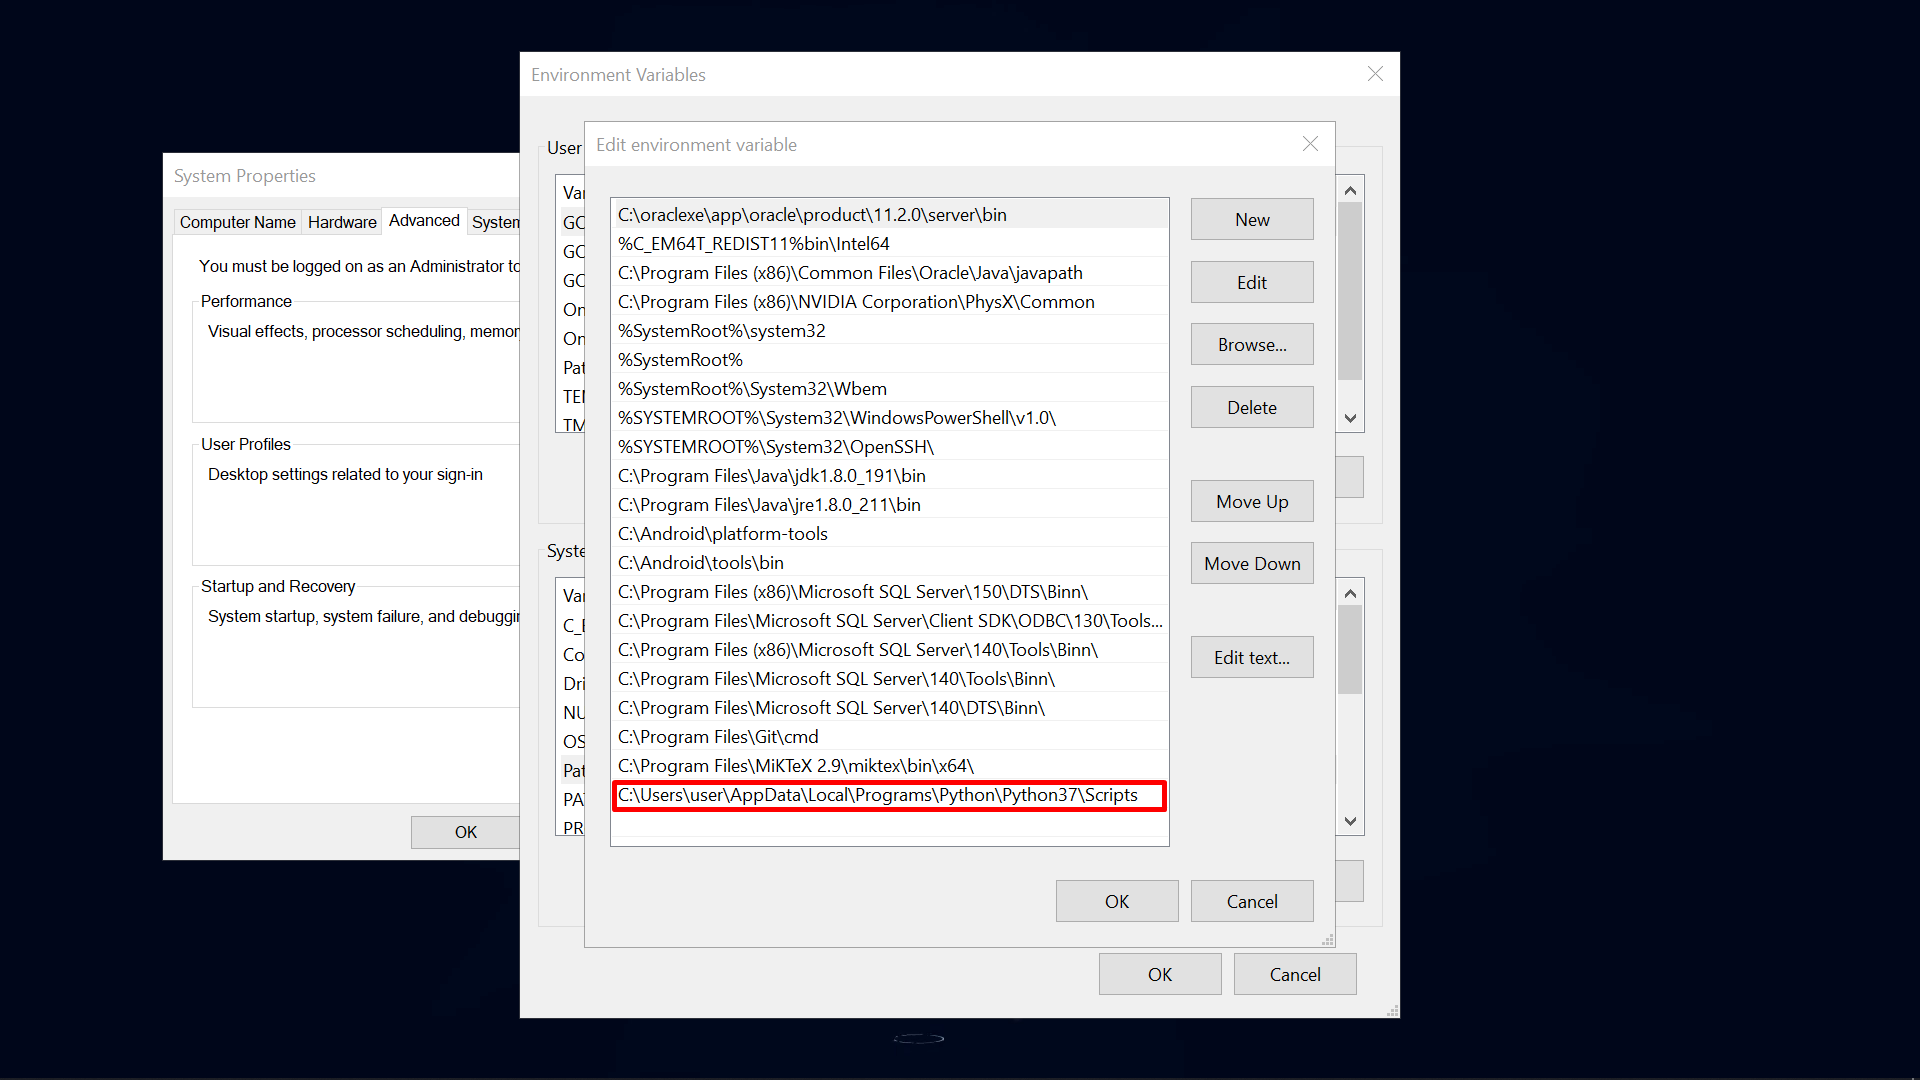
\includegraphics[width=10cm]{figures/envi4.png}
	\caption{Add Environments}
\end{figure}
\end{itemize}

\section{Entrepreter/cli Melalui Terminal atau CMD Windows}
\begin{itemize} 
\item Entrepreter di CMD.
\begin{figure}[!htbp]
	\centering
	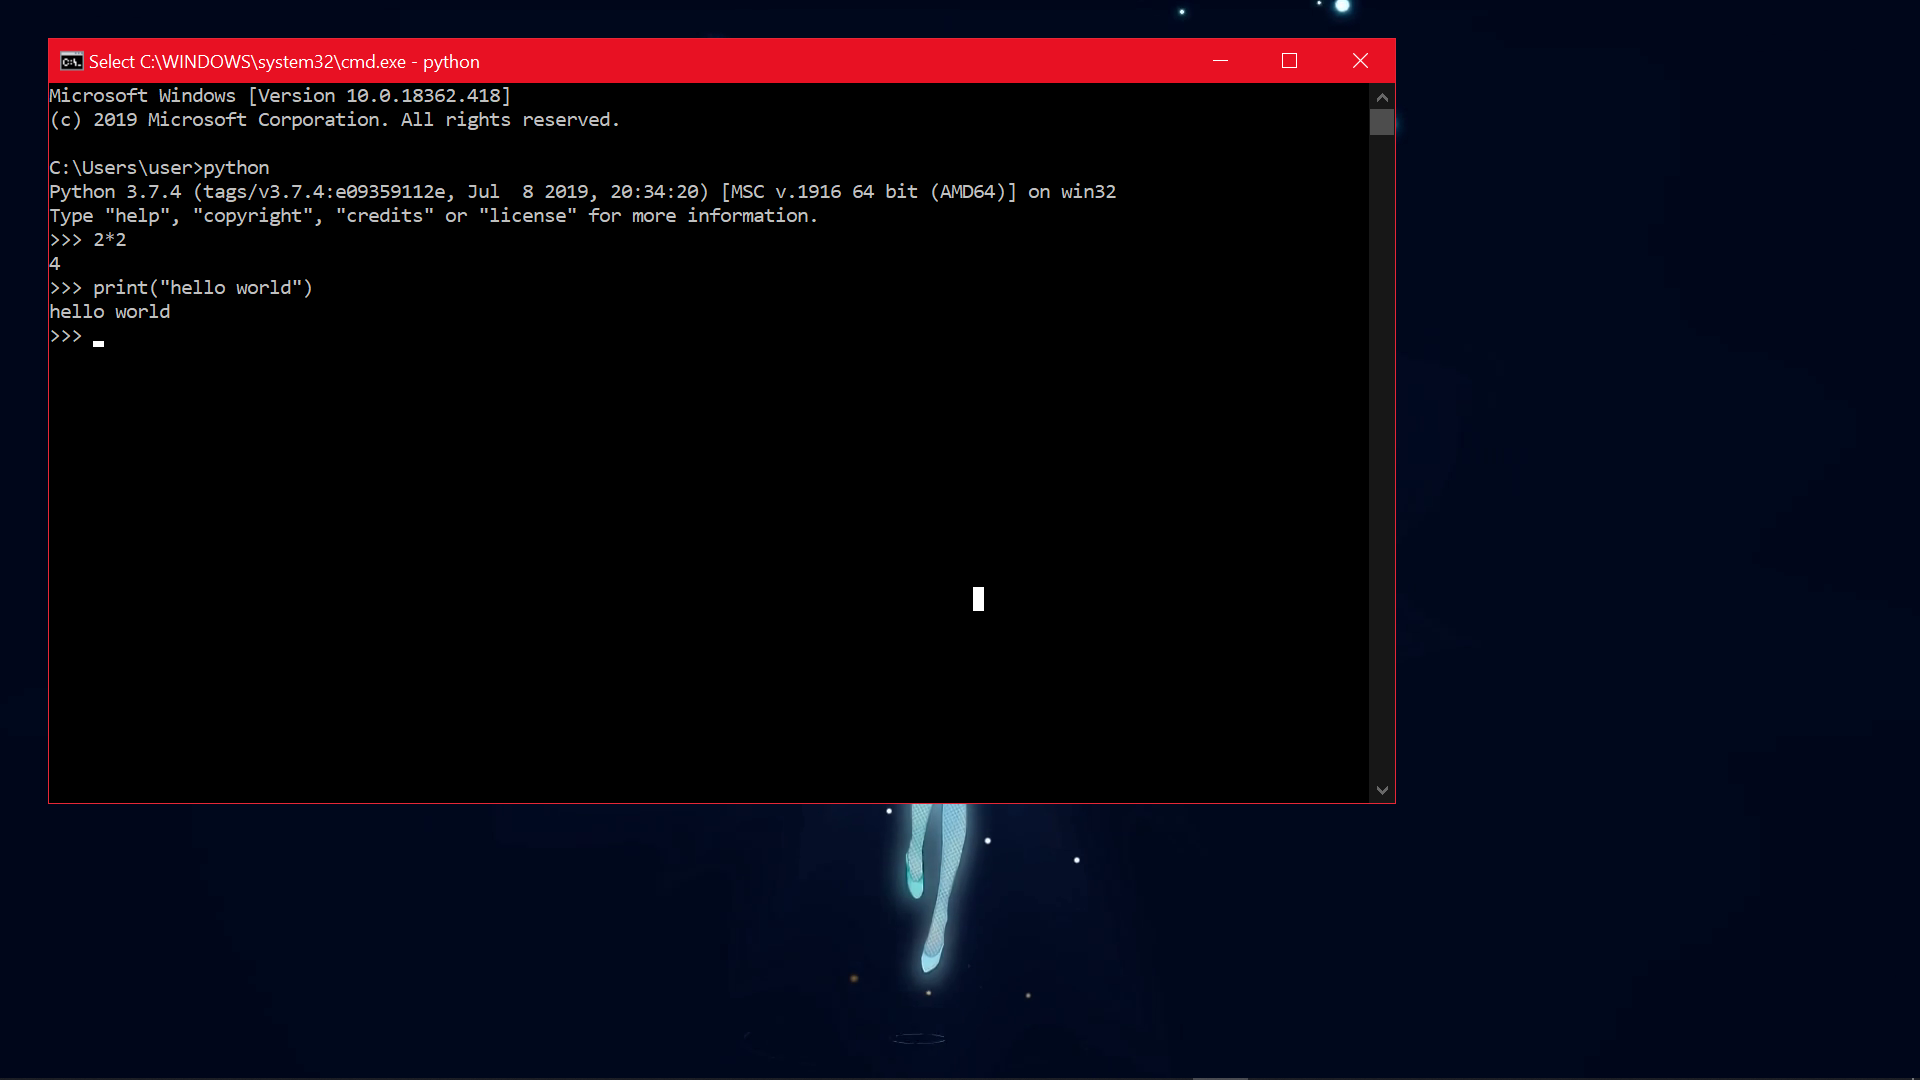
\includegraphics[width=10cm]{figures/enterpreter.png}
	\caption{Enterpreter Python di CMD}
\end{figure}
\end{itemize}

\section{Menjalankan dan Mengupdate Anaconda dan Spyder}
Karena anaconda telah terinstall kini kita tinggal menjalankannya saja.

\begin{itemize}
\item Buka CMD dan ketik "conda install -c conda-forge basemap" lalu enter. Tunggu proses sampai selesai.
\begin{figure}[!htbp]
	\centering
	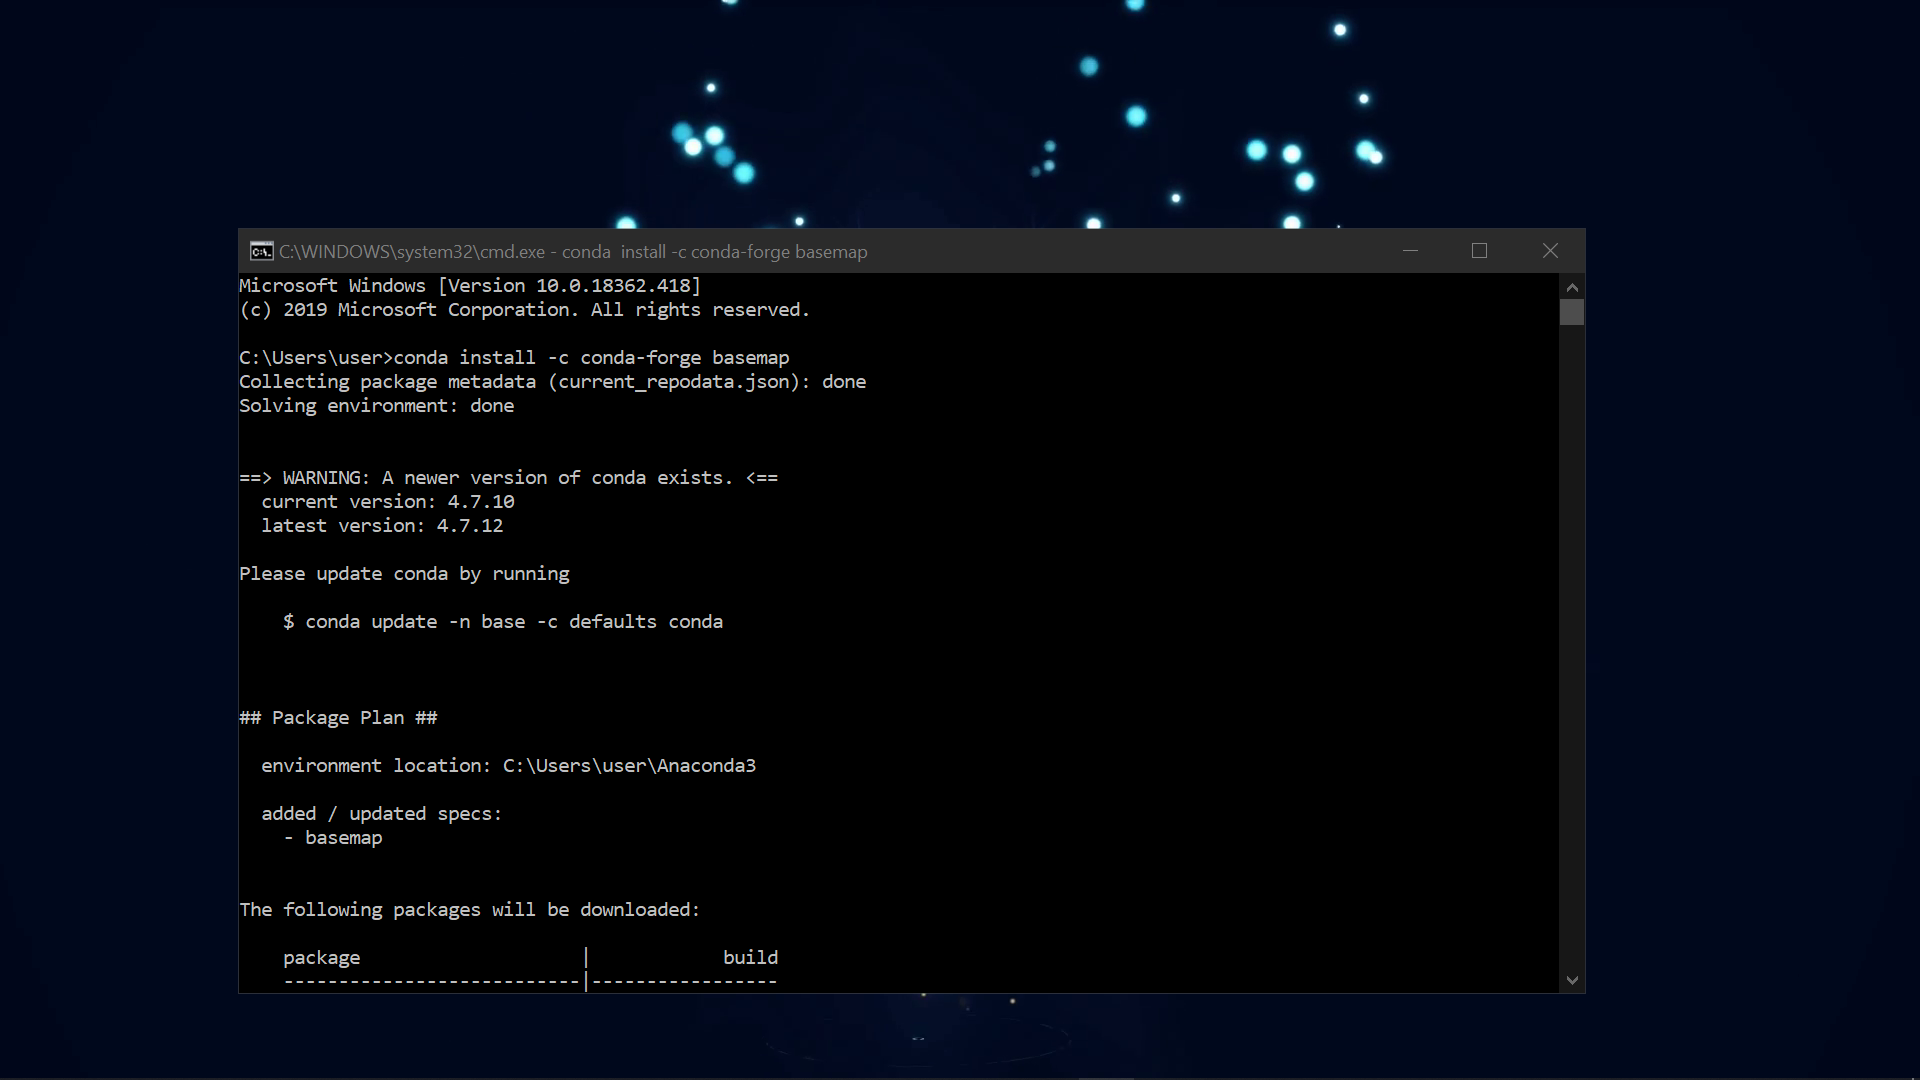
\includegraphics[width=10cm]{figures/conda1.png}
	\caption{Install conda forge basemap}
\end{figure}
\item Setelah proses selesai akan muncul tampilan seperti di bawah, ketik "y" lalu enter, tunggu sampai proses download selesai.
\begin{figure}[!htbp]
	\centering
	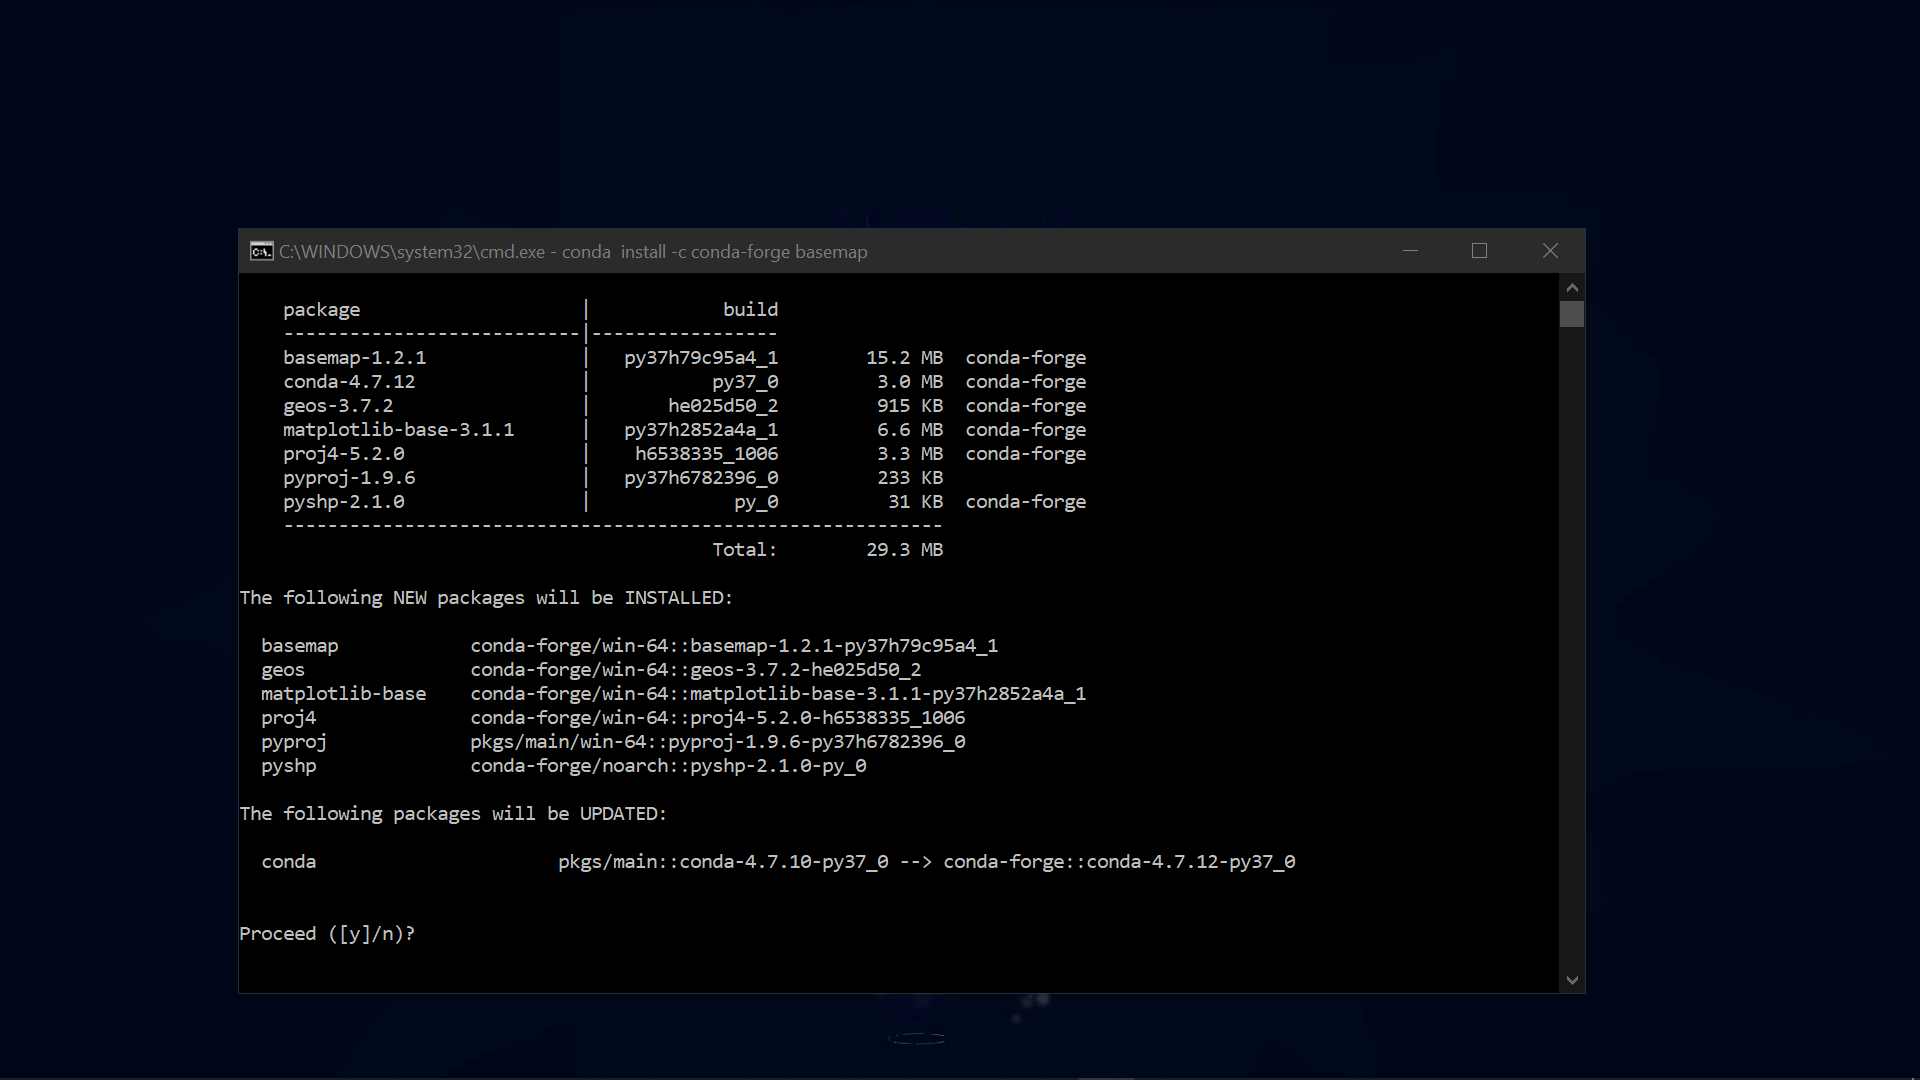
\includegraphics[width=10cm]{figures/conda2.png}
	\caption{Download dan Extract Packages}
\end{figure}
\item Setelah proses install selesai masuk lagi ke cmd python. Lalu ketik "impert geopy". Jika file tidak ditemukan berarti file tidak ada. Untuk mengatasi masalah tersebut ketik di cmd "pip install geopy memory_profiler".
\begin{figure}[!htbp]
	\centering
	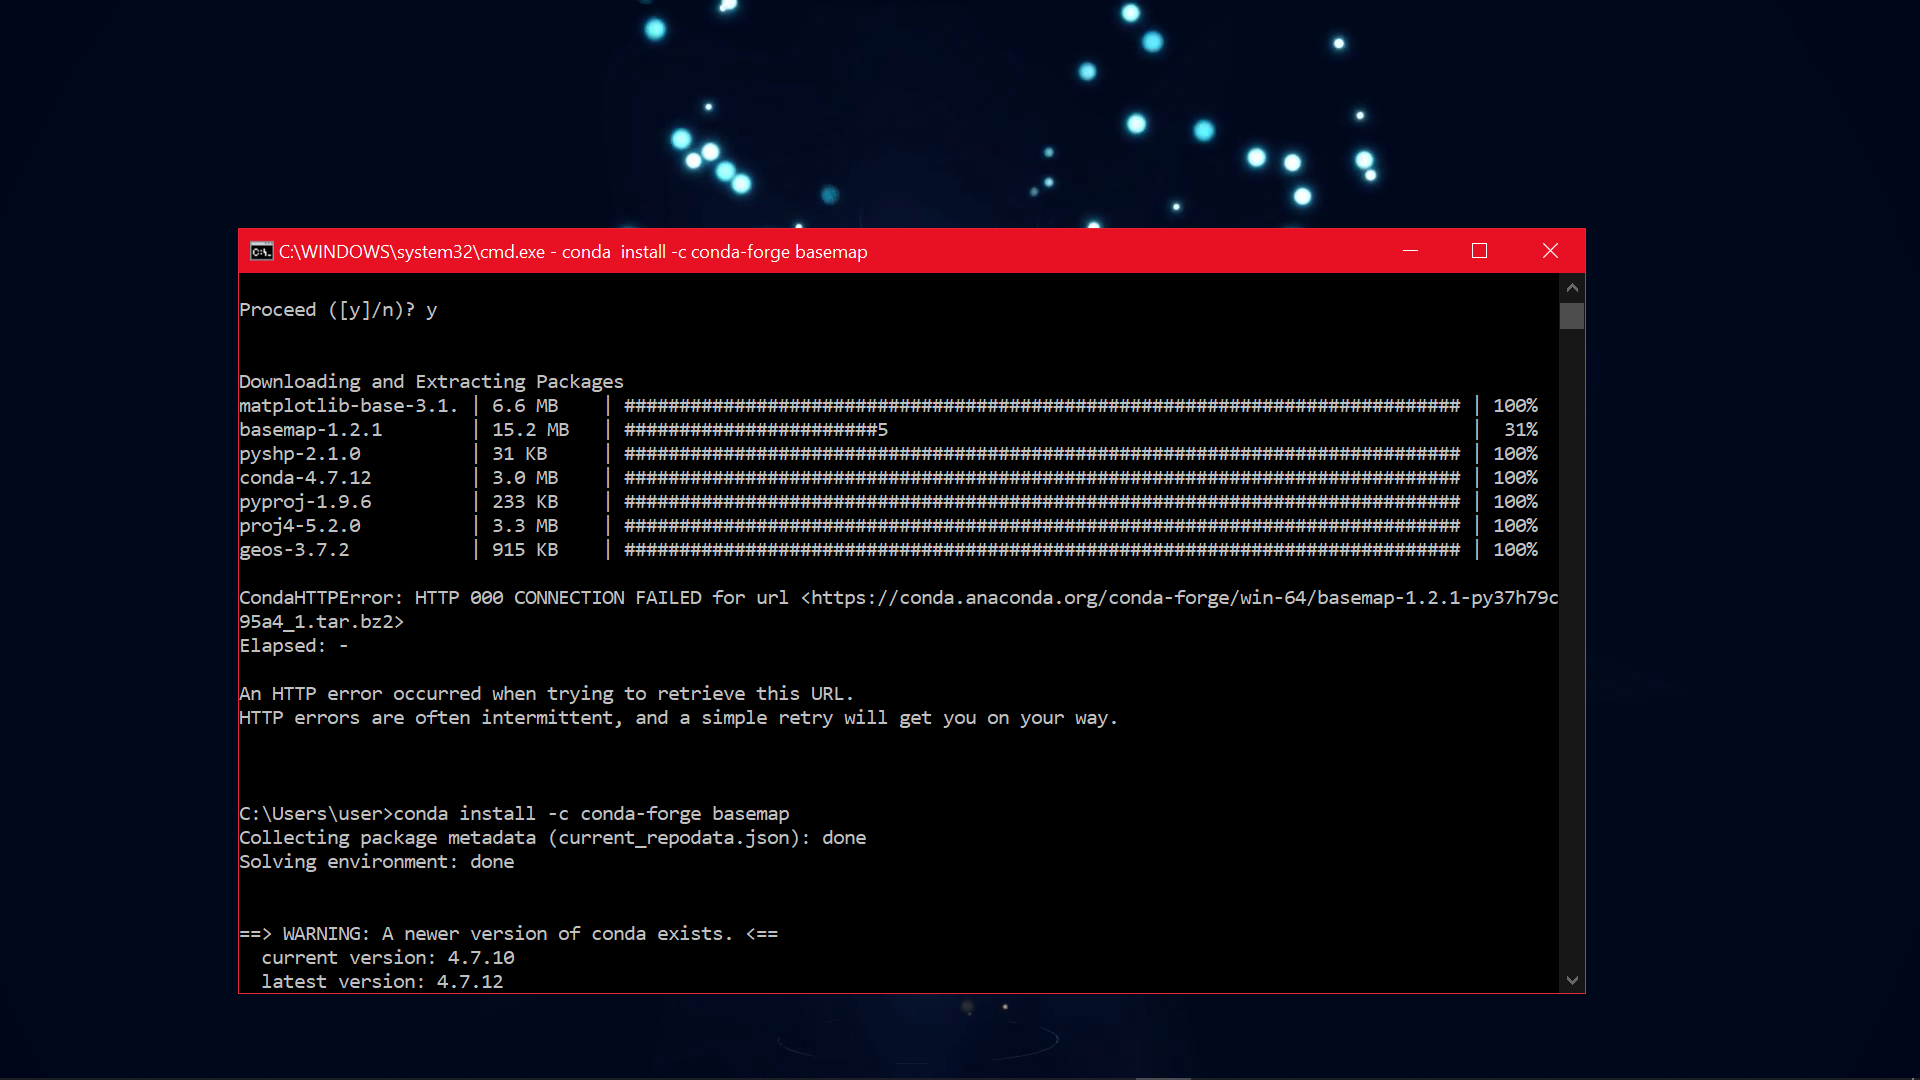
\includegraphics[width=10cm]{figures/conda3.png}
	\caption{Install Geopy}
\end{figure}
\item Tunggu sampai selesai, jika sudah selesai masuk lagi ke cmd python lalu ketik "import geopy" dan geopy akan ter-import.
\begin{figure}[!htbp]
	\centering
	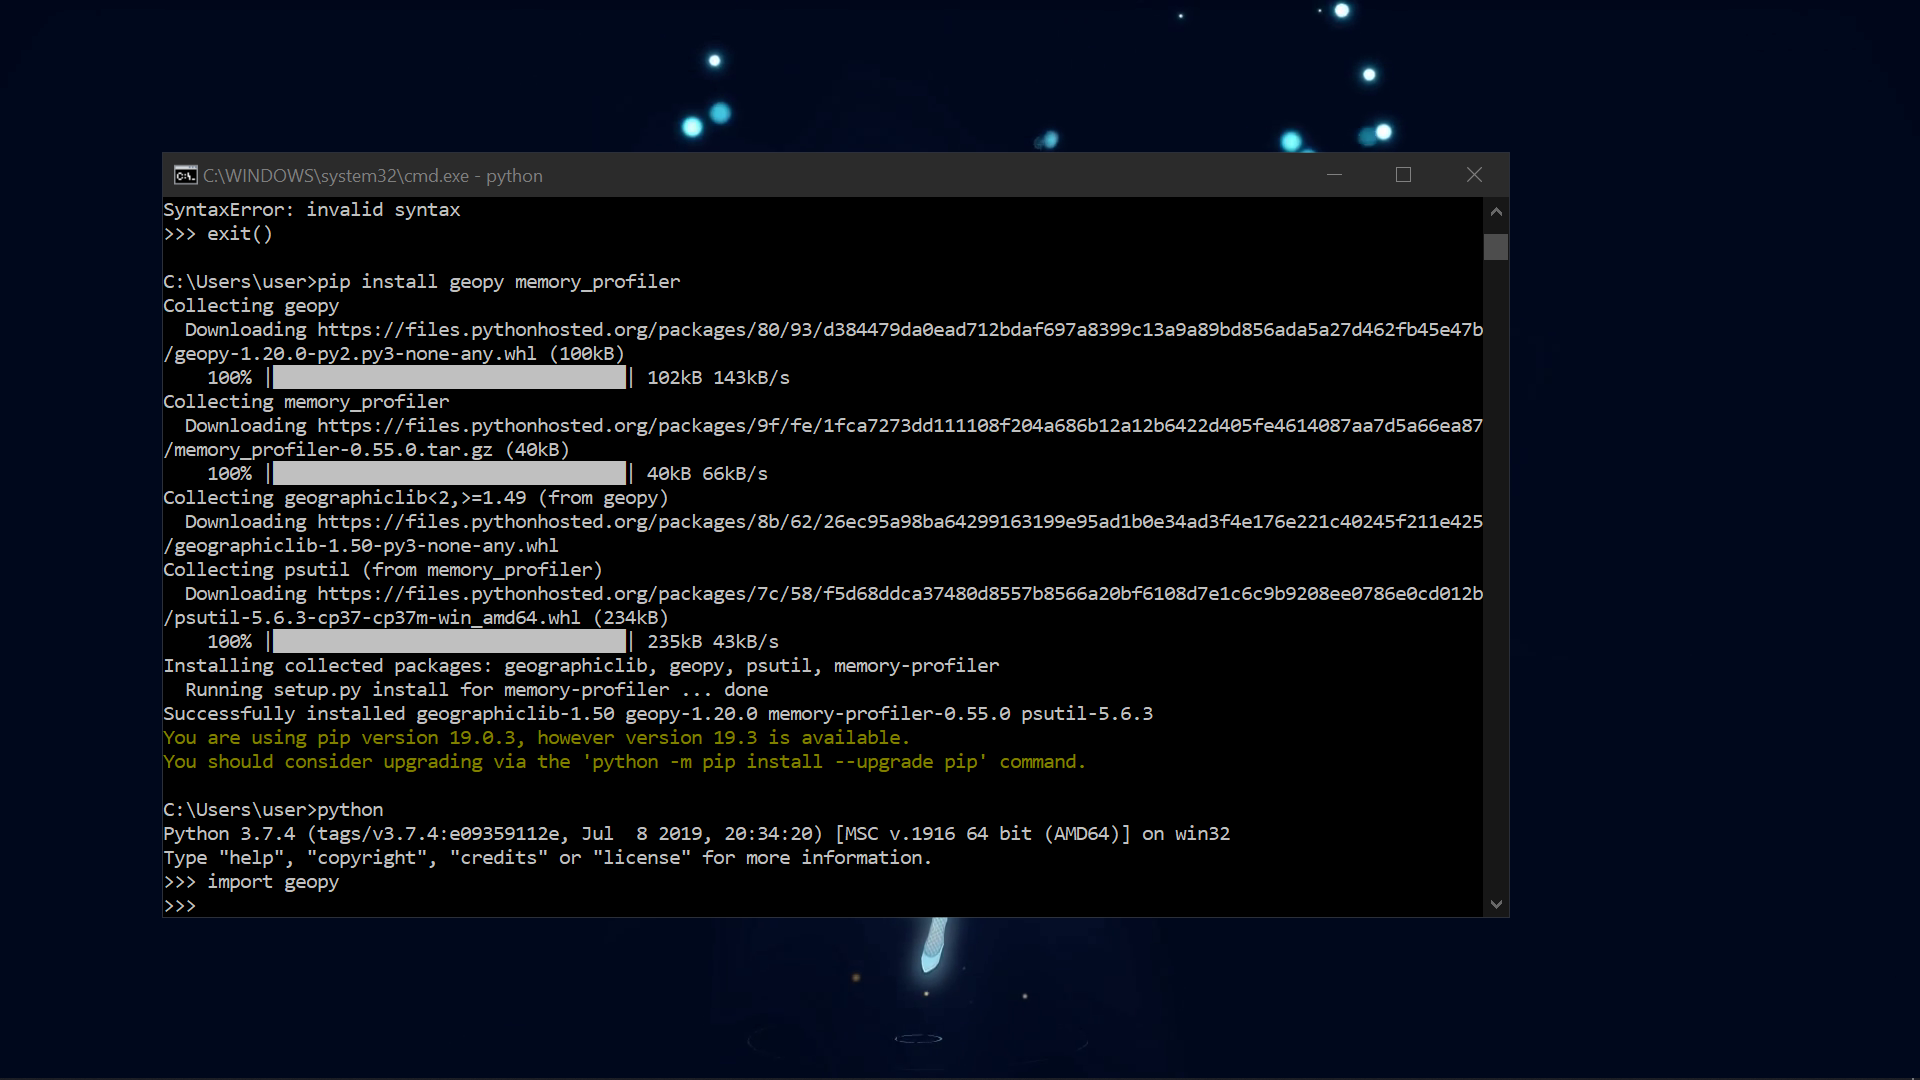
\includegraphics[width=10cm]{figures/conda4.png}
	\caption{Import Geopy}
\end{figure}
\item Buka anaconda.
\begin{figure}[!htbp]
	\centering
	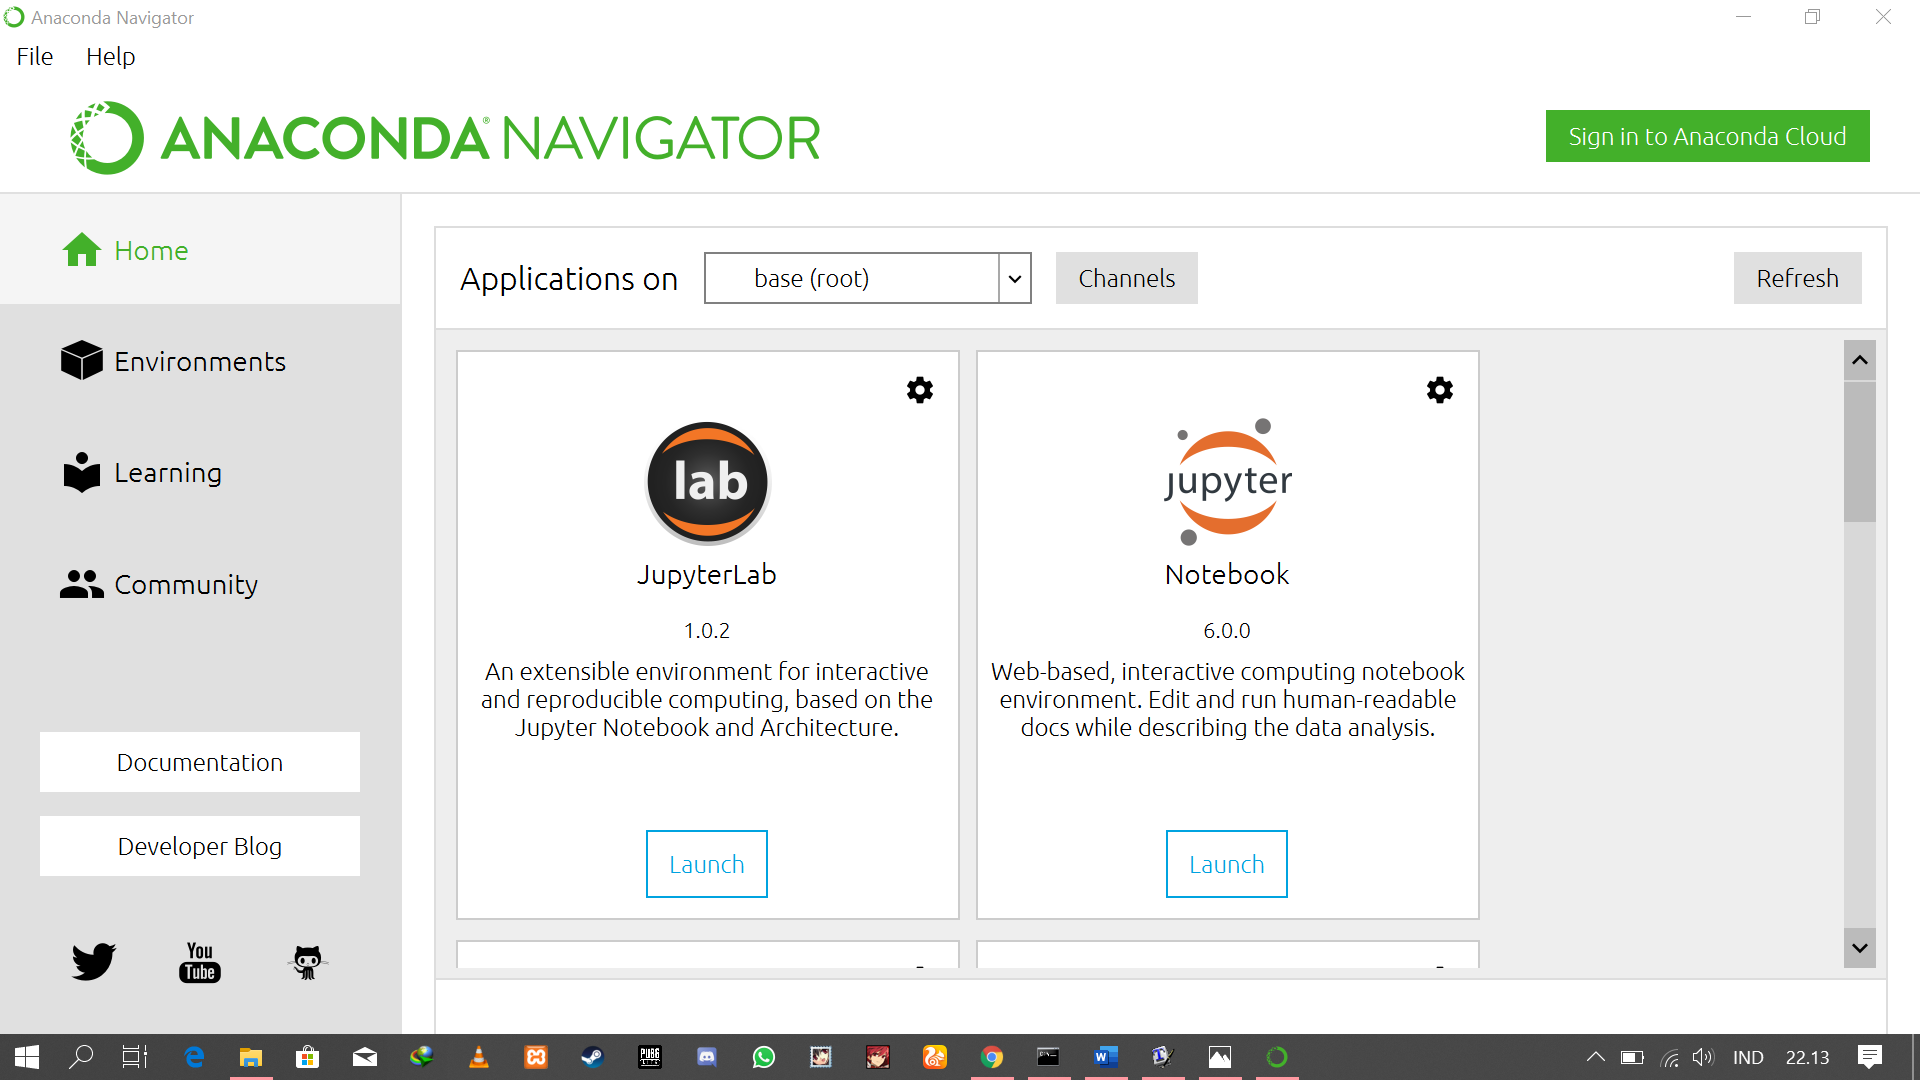
\includegraphics[width=10cm]{figures/conda5.png}
	\caption{Tampilan Anaconda3}
\end{figure}
\item Buka Spyder.
\begin{figure}[!htbp]
	\centering
	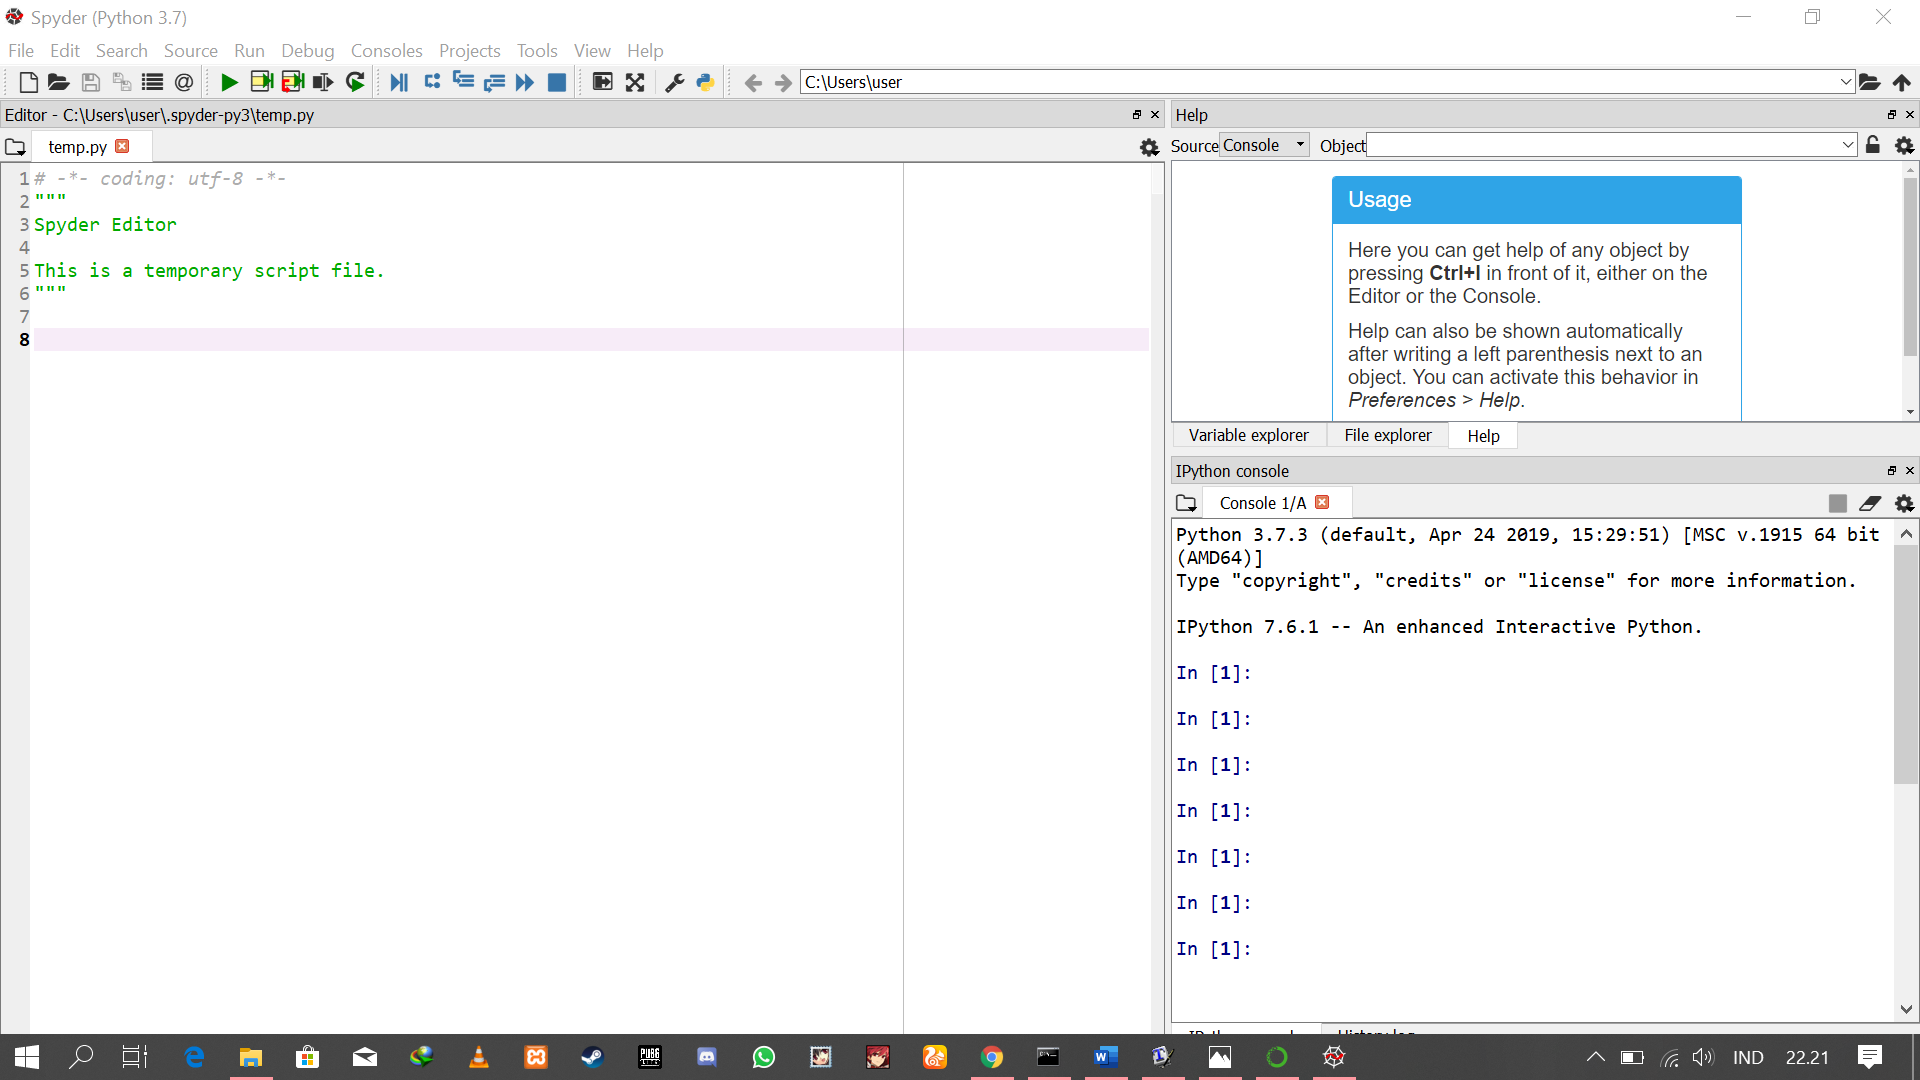
\includegraphics[width=10cm]{figures/conda6.png}
	\caption{Tampilan Spyder}
\end{figure}
\end{itemize}

\section{Cara Menjalankan Script Hello Word di Spyder}
\begin{itemize}
\item Buka Spyder.
\begin{figure}[!htbp]
	\centering
	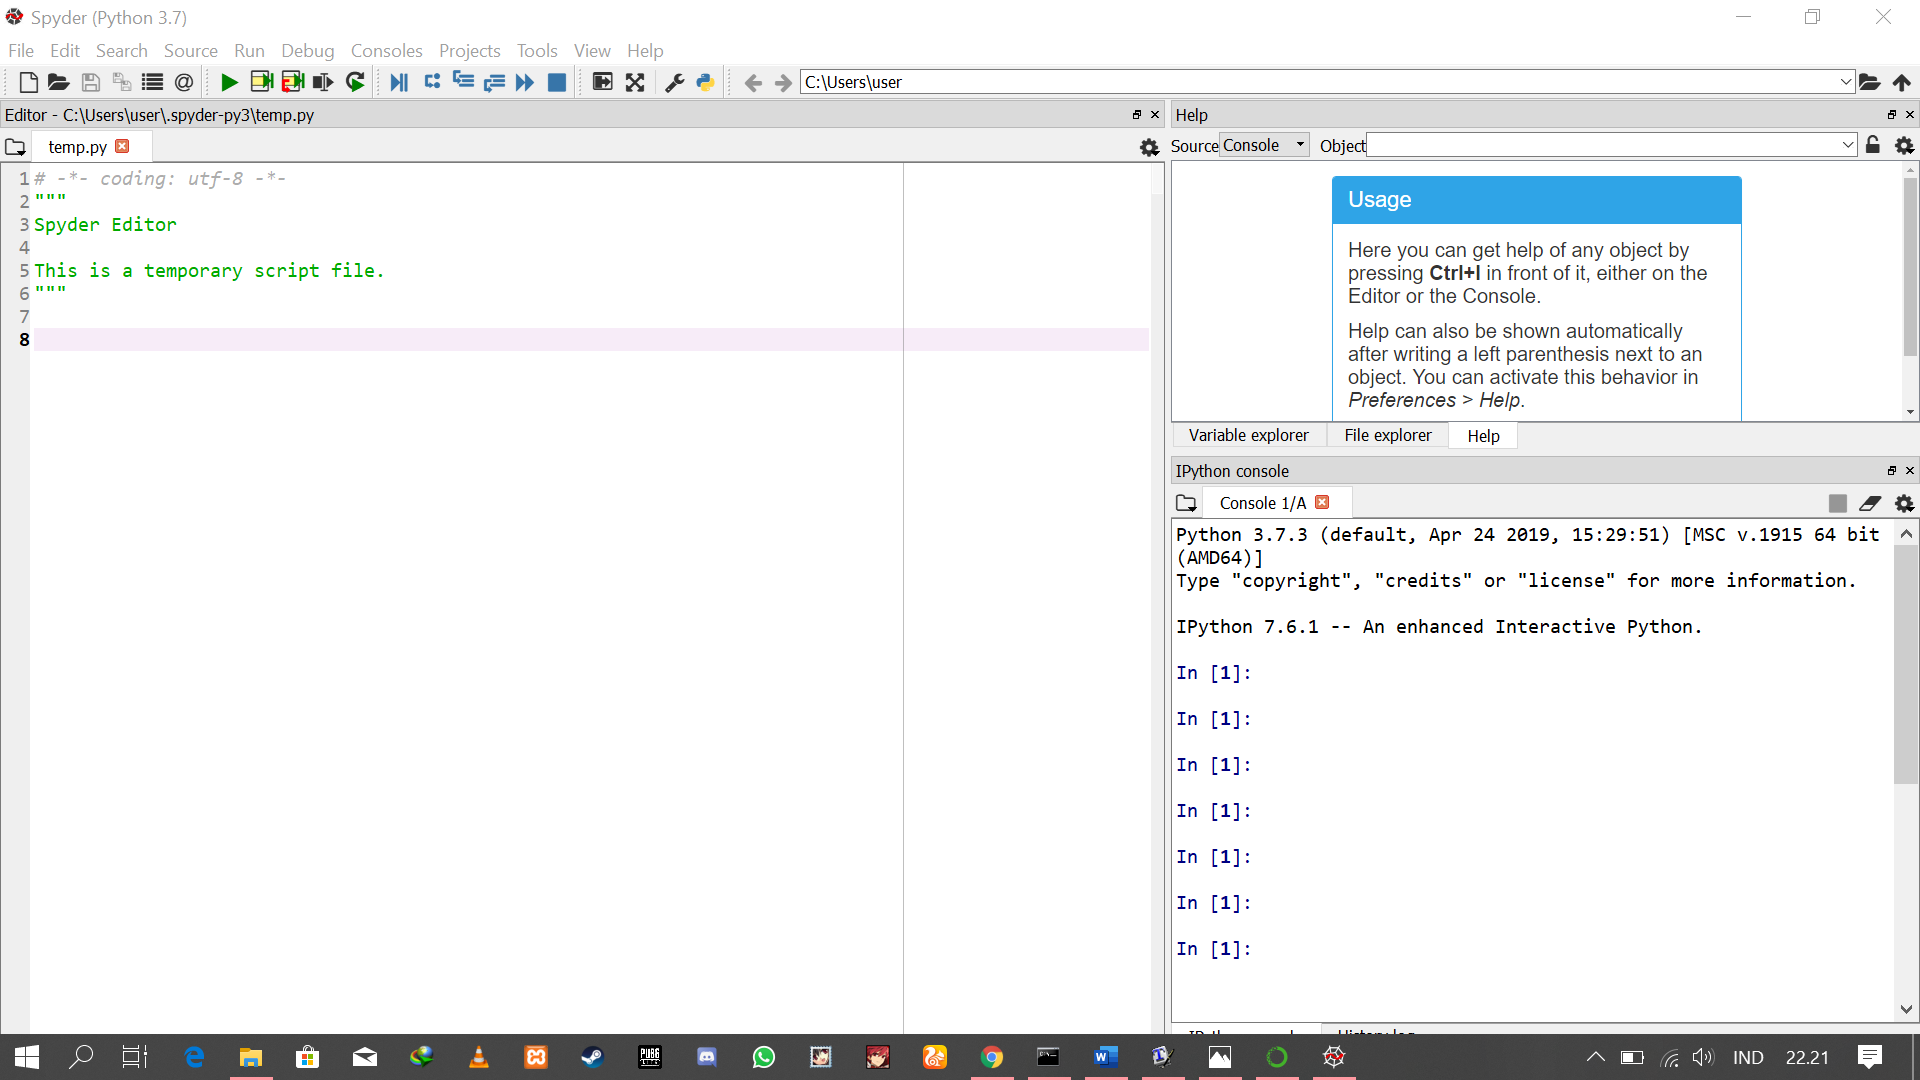
\includegraphics[width=10cm]{figures/conda6.png}
	\caption{Tampilan Spyder}
\end{figure}
\item Tulis print(“hello world”) dan runing dengan memilih run file dengan cara f5 hasil nya dapat dilihat pada ipython console.
\begin{figure}[!htbp]
	\centering
	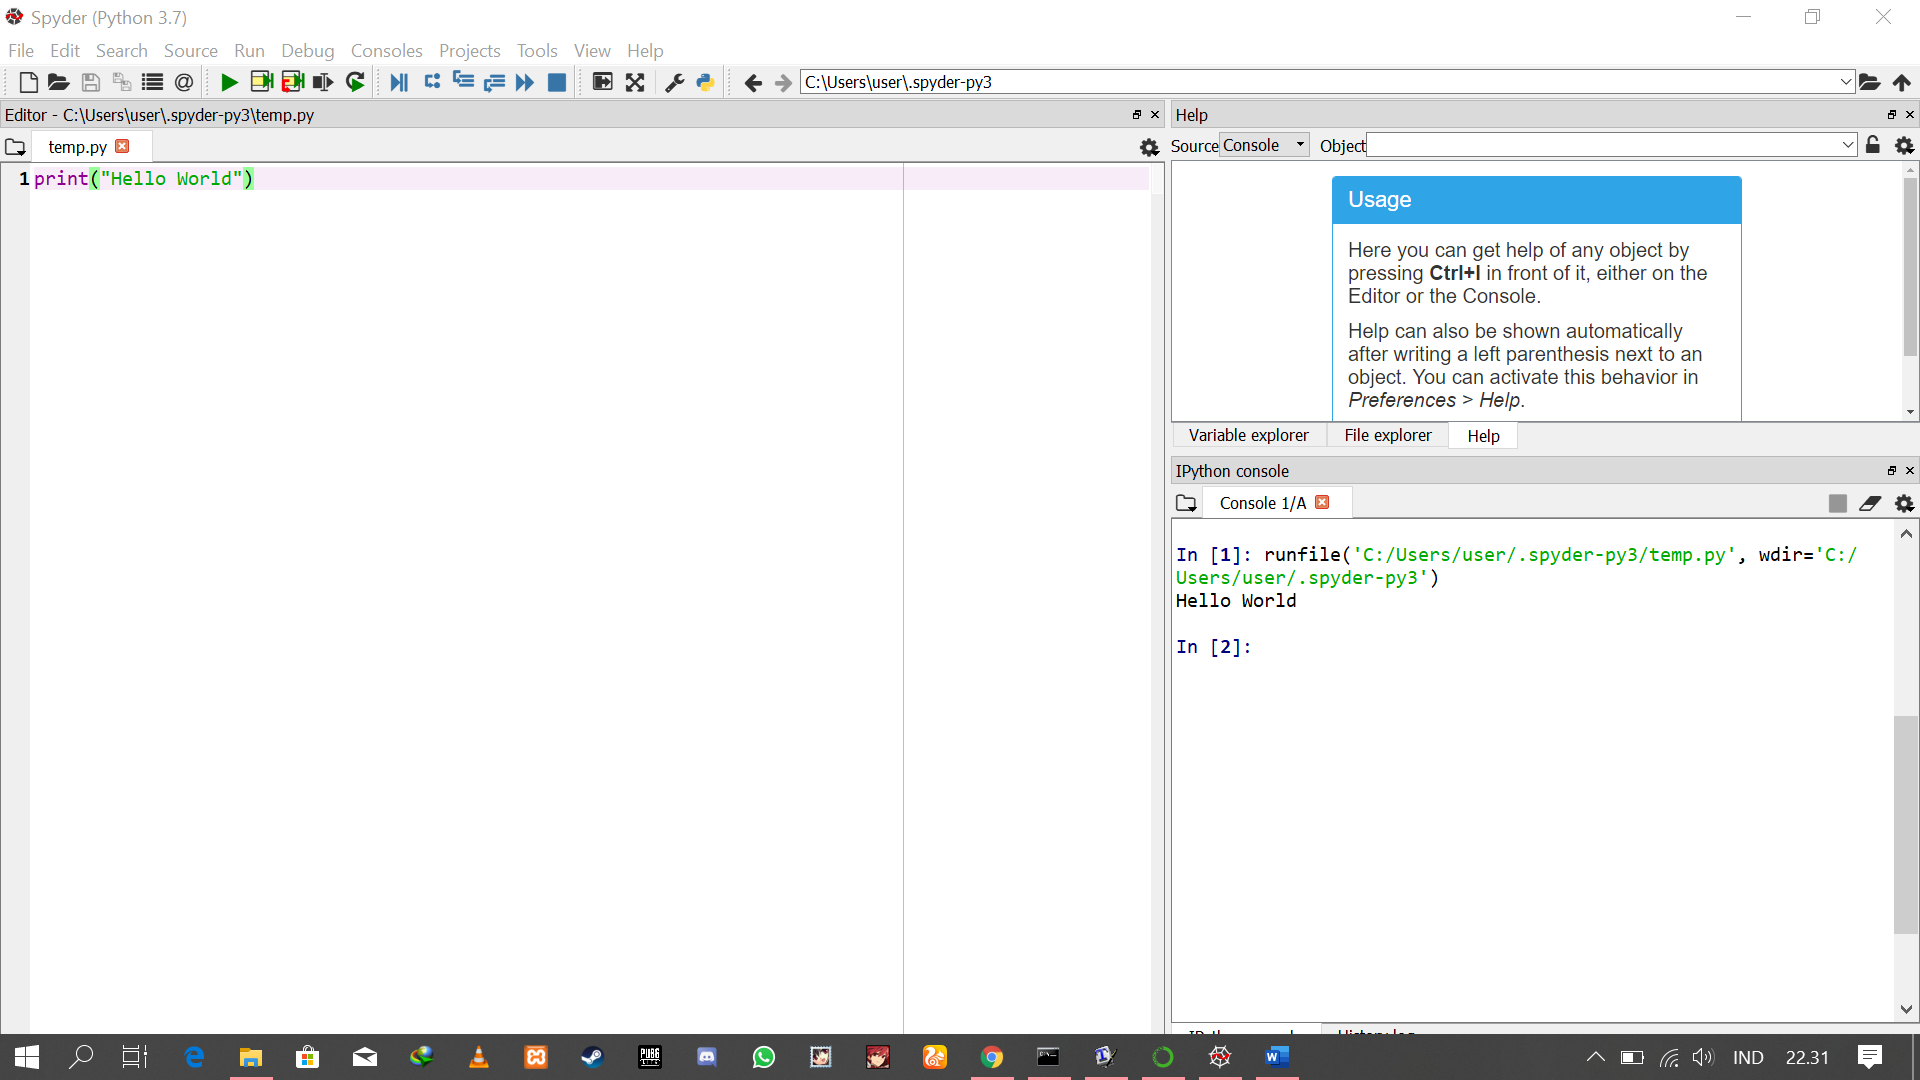
\includegraphics[width=10cm]{figures/conda7.png}
	\caption{Tampilan Spyder}
\end{figure}
\end{itemize}

\section {Cara Menjalankan Script Otomatis Login Aplikasi Akademik dengan Library Selenium dan Inputan User}
Selenium adalah alat untuk menguji aplikasi web Anda. Anda dapat melakukan ini dengan berbagai cara, misalnya:

\begin{itemize}
\item Izinkan untuk mengetuk tombol
\item Masukkan konten dalam struktur
\item Telusuri situs Anda untuk memeriksa apakah semuanya "OK" dan seterusnya.
\end{itemize}
Berikut adalah contoh penggunaan selenium.
\begin{itemize}
\item Pertama-tama install selenium webdriver. Jika sudah ter-install langsung saja tulis skrip pada gambar di bawah. Lalu simpan dengan fb.py.
\begin{figure}[!htbp]
	\centering
	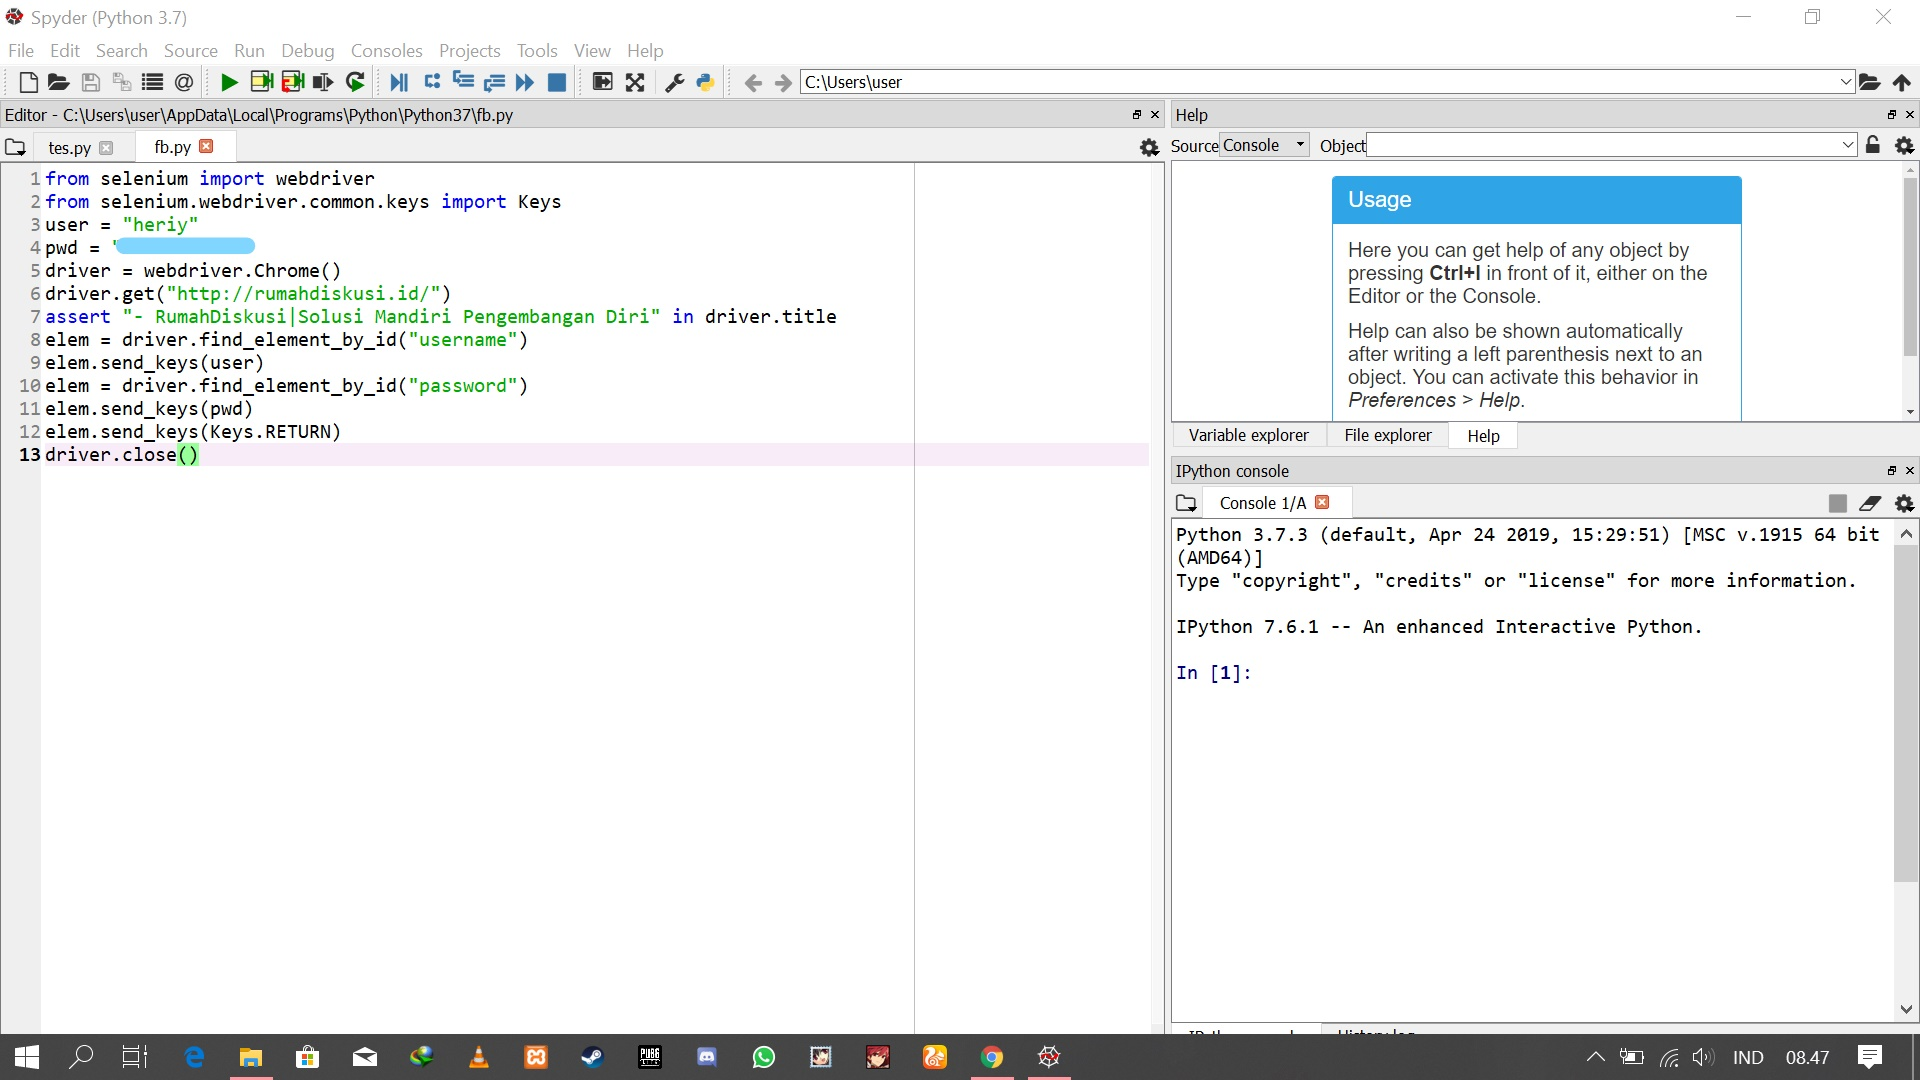
\includegraphics[width=10cm]{figures/selenium10.jpg}
	\caption{Selenium Skrip}
\end{figure}
\item Jika sudah buka command promt tempat anda menyimpan file fb.py. Lalu ketik python fb.py lalu tekan enter.
\begin{figure}[!htbp]
	\centering
	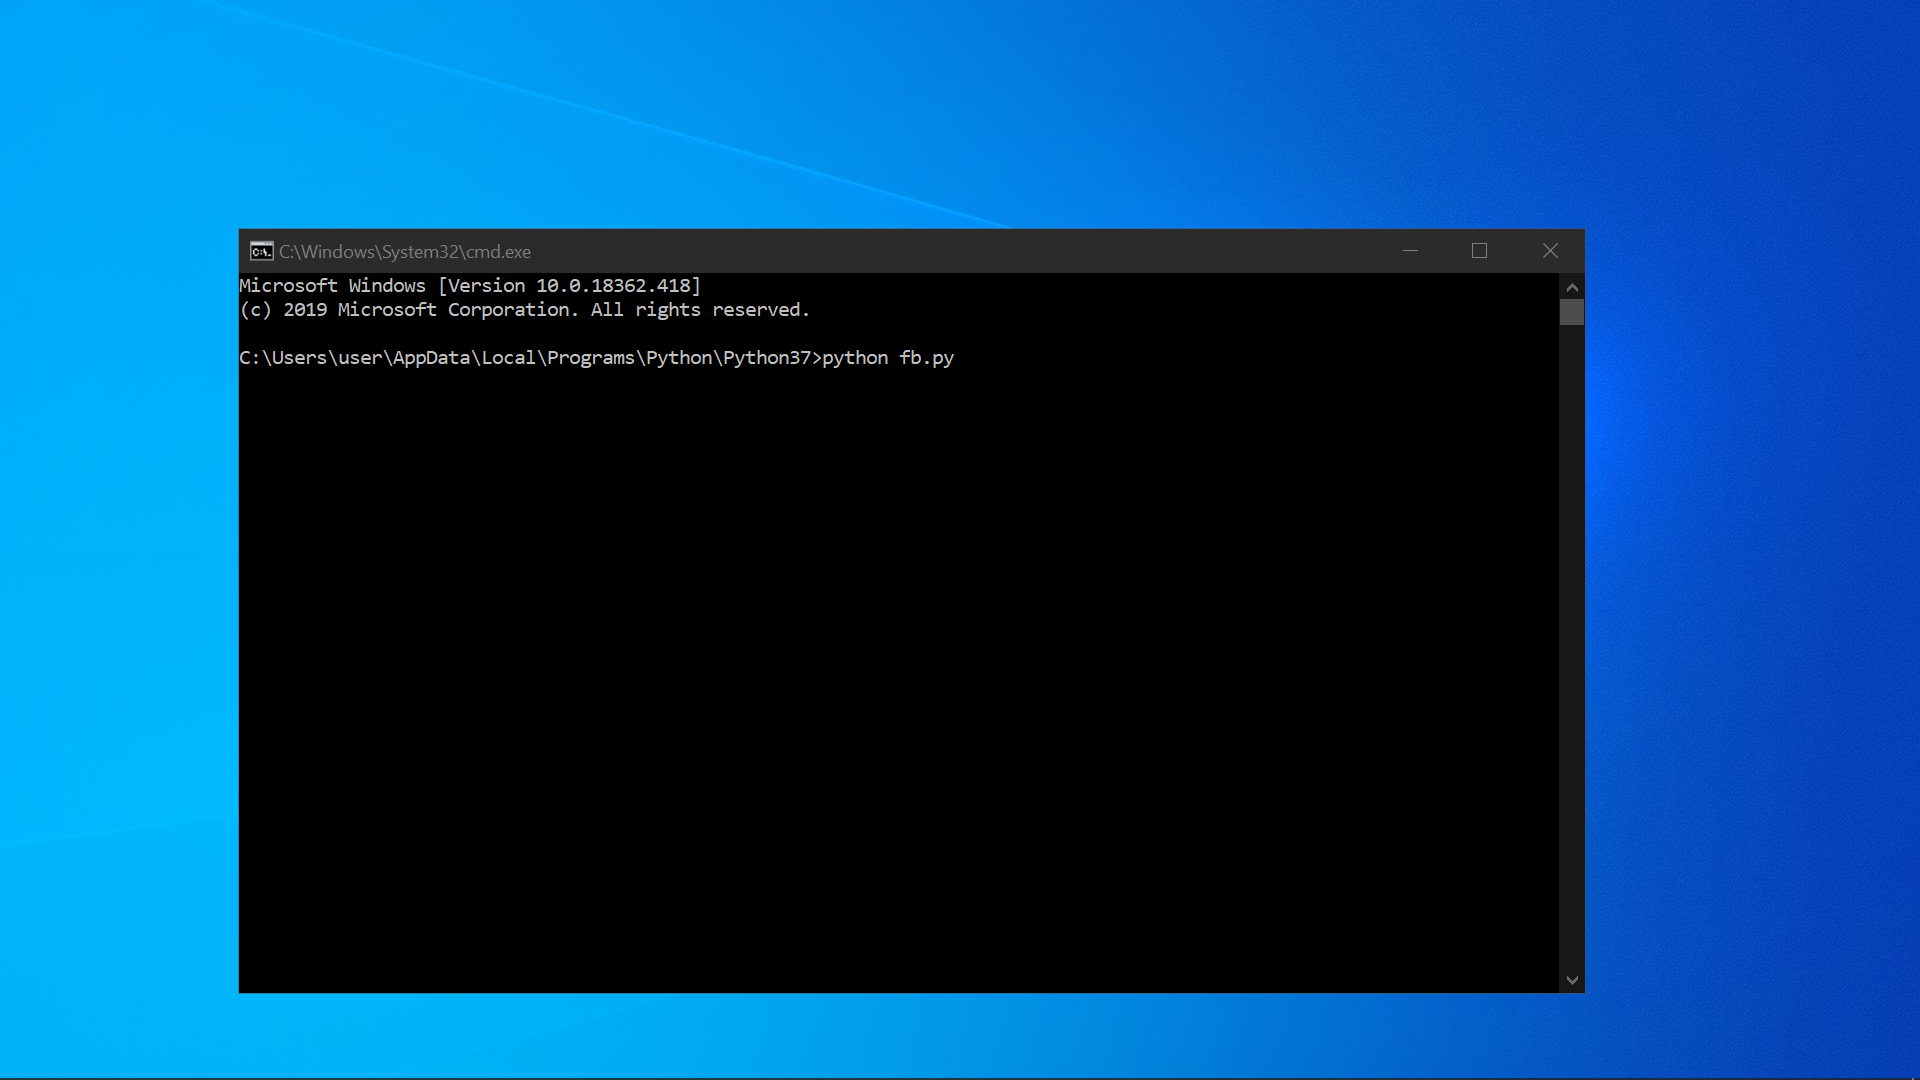
\includegraphics[width=10cm]{figures/selenium11.png}
	\caption{Command Prompt}
\end{figure}
\item Jika berhasil akan muncul browser, seperti pada gambar di bawah.
\begin{figure}[!htbp]
	\centering
	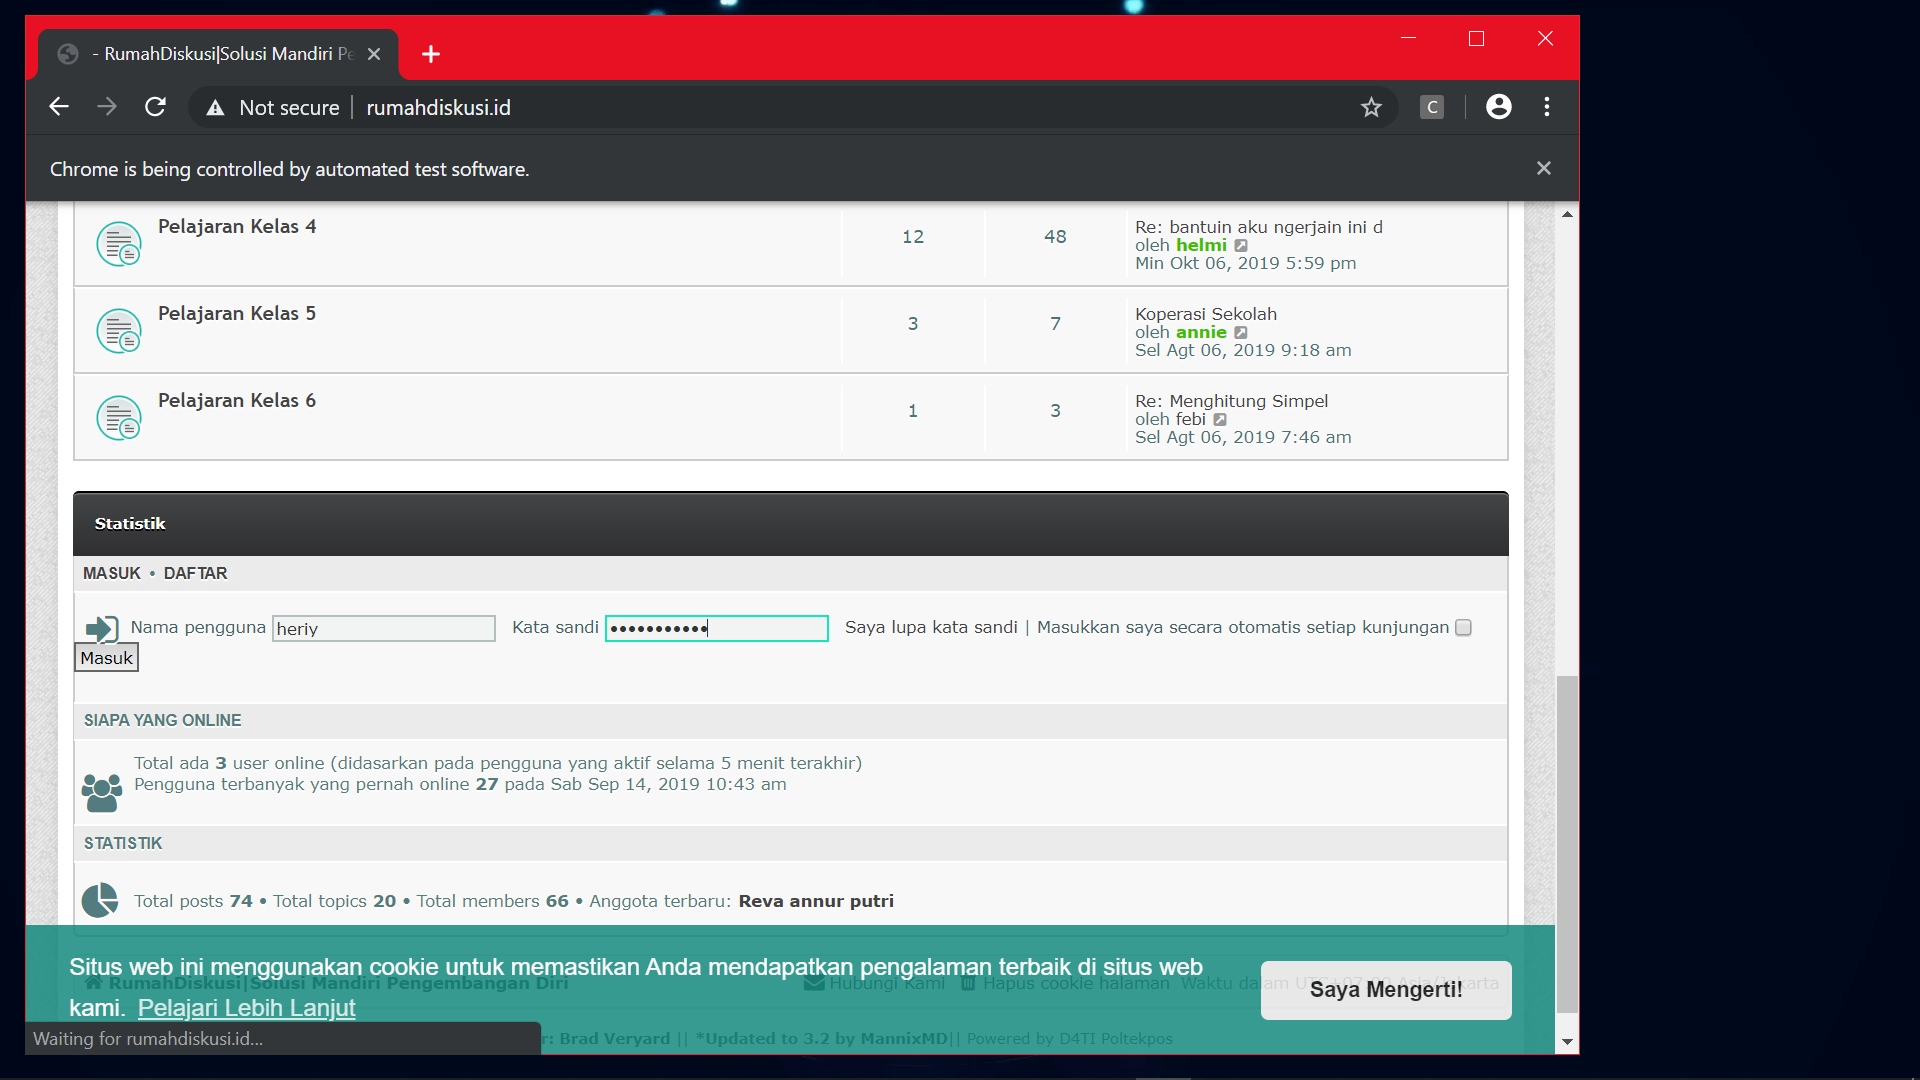
\includegraphics[width=10cm]{figures/selenium7.png}
	\caption{Rumah Diskusi}
\end{figure}
\item Halaman Rumah Diskusi.
\begin{figure}[!htbp]
	\centering
	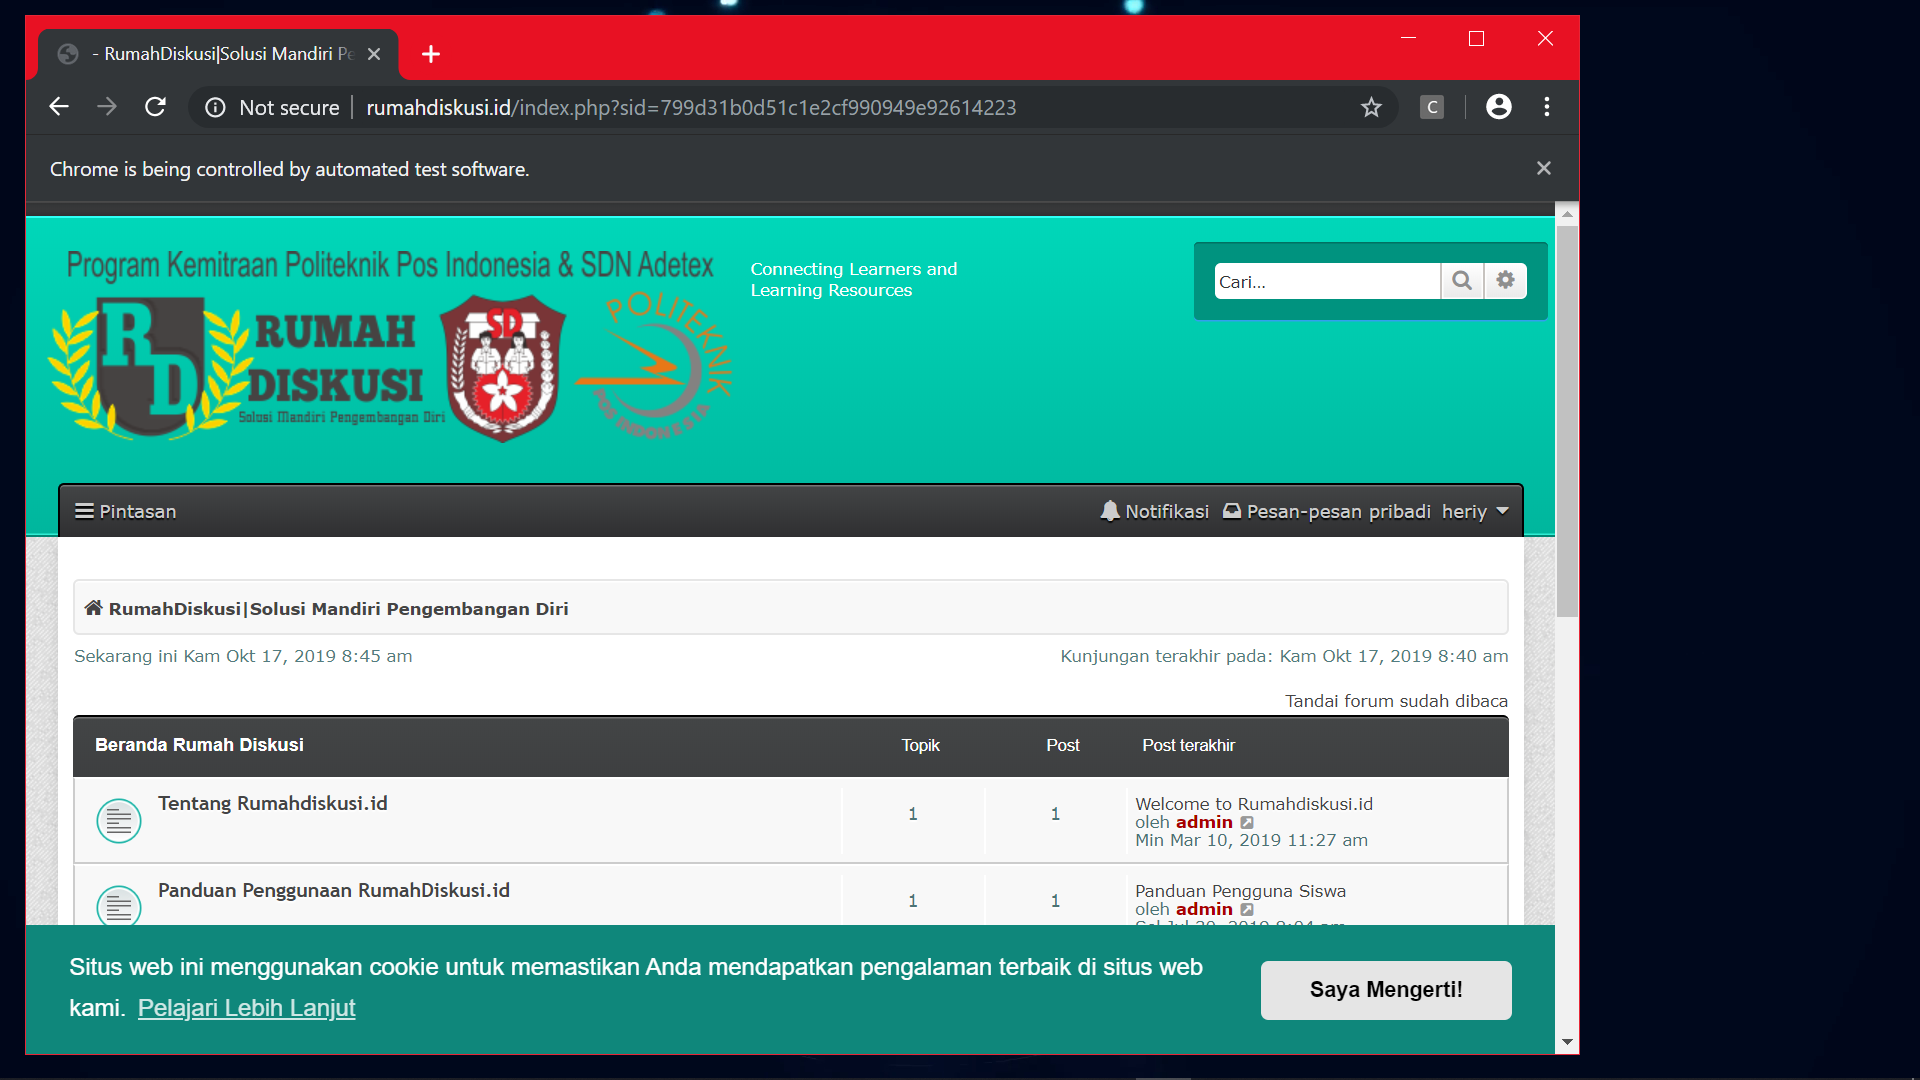
\includegraphics[width=10cm]{figures/selenium8.png}
	\caption{Rumah Diskusi}
\end{figure}
\end{itemize}

\subsection{Pemakaian Variable Explorer di Spyder}
Variable explorer di spyder berfungsi untuk mengidentifikasi nama variable, tipe data variable, ukuran variable, dan nilai dari variable yang dimasukkan ke dalam script. Lihat gambar di bawah ini.
\begin{figure}[!htbp]
	\centering
	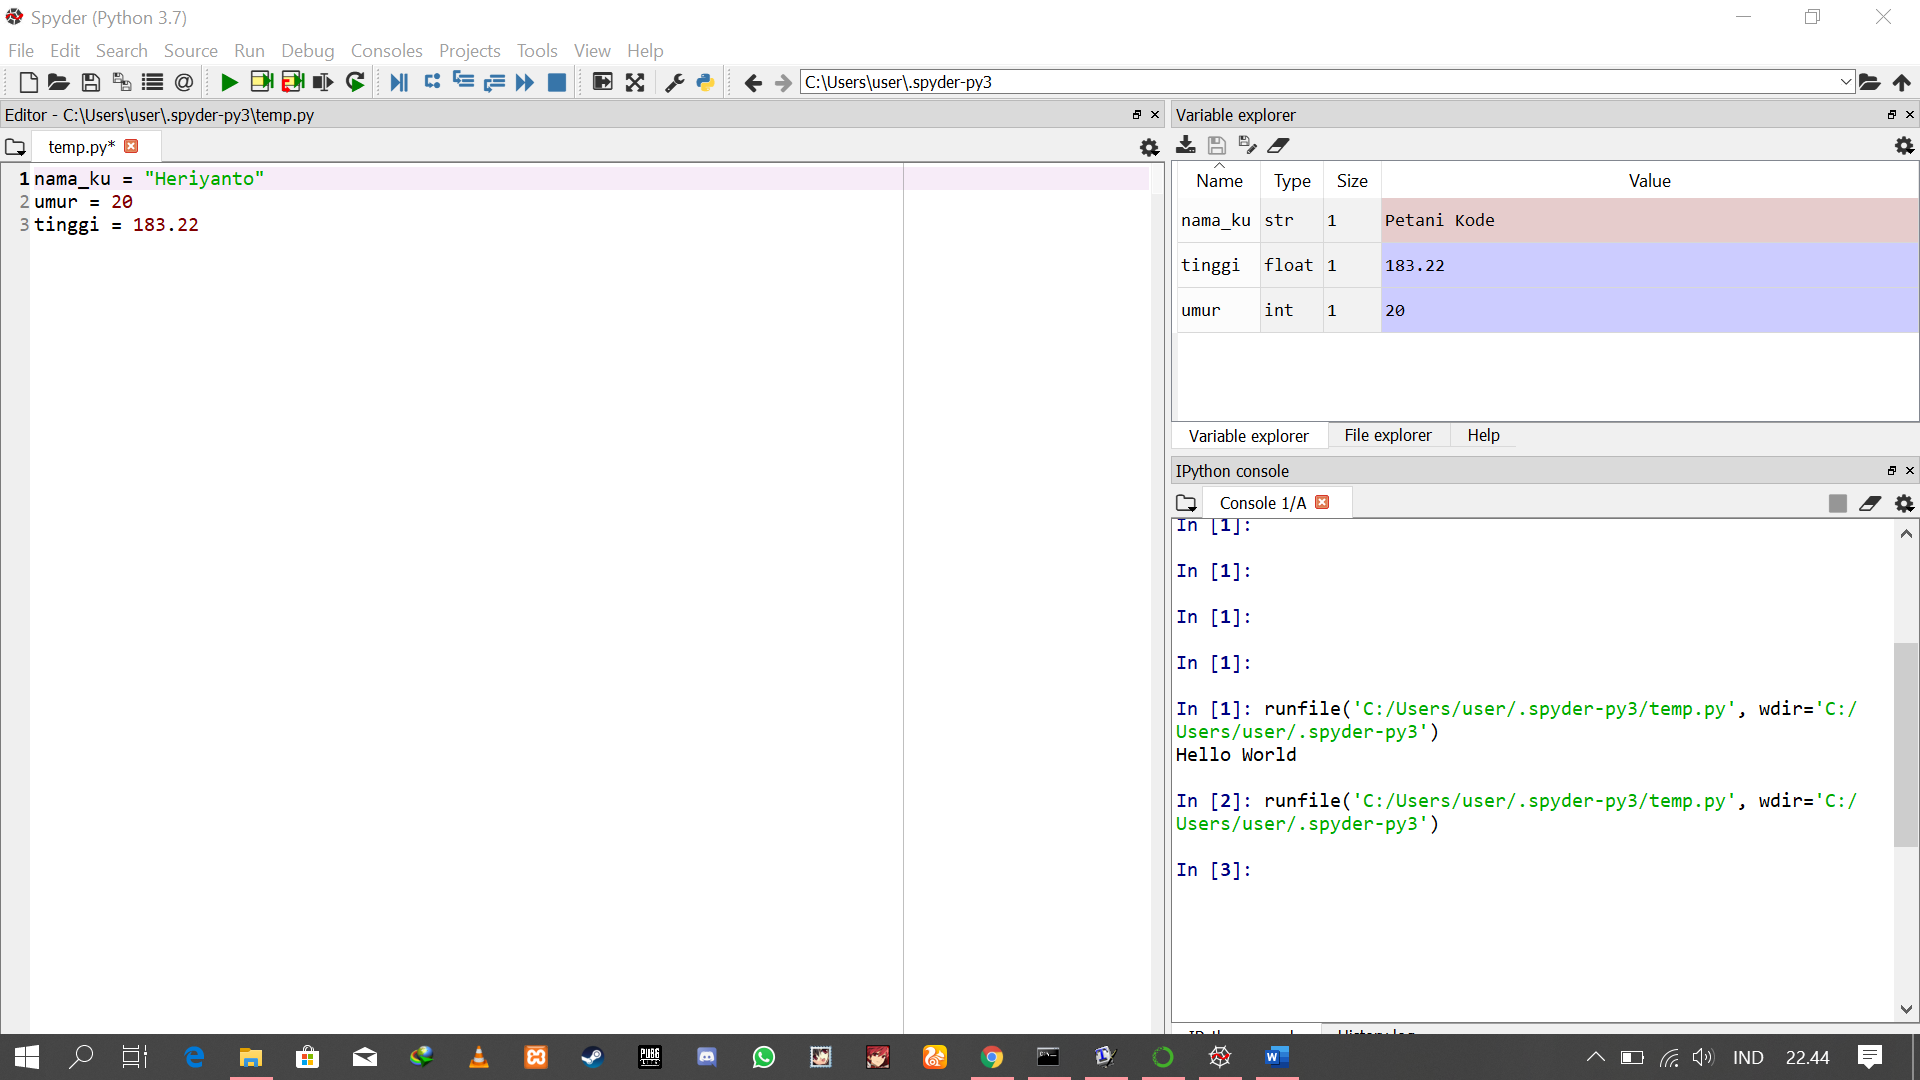
\includegraphics[width=10cm]{figures/varex.png}
	\caption{Variable Explorer}
\end{figure}
\end{document}